\documentclass[preprint,12pt]{elsarticle}

%% Use the option review to obtain double line spacing
%% \documentclass[authoryear,preprint,review,12pt]{elsarticle}

%% Use the options 1p,twocolumn; 3p; 3p,twocolumn; 5p; or 5p,twocolumn
%% for a journal layout:
%% \documentclass[final,1p,times]{elsarticle}
%% \documentclass[final,1p,times,twocolumn]{elsarticle}
%% \documentclass[final,3p,times]{elsarticle}
%% \documentclass[final,3p,times,twocolumn]{elsarticle}
%% \documentclass[final,5p,times]{elsarticle}
%% \documentclass[final,5p,times,twocolumn]{elsarticle}

%% For including figures, graphicx.sty has been loaded in
%% elsarticle.cls. If you prefer to use the old commands
%% please give \usepackage{epsfig}

%% The amssymb package provides various useful mathematical symbols
\usepackage{amssymb}
%% The amsmath package provides various useful equation environments.
%% The amsthm package provides extended theorem environments
%% \usepackage{amsthm}
\usepackage{amsmath,amsfonts}
\usepackage{algorithm}
\usepackage{array}
\usepackage{makecell}
\usepackage{textcomp}

%\usepackage{stfloats}
%\usepackage[caption=false,font=normalsize,labelfont=sf,textfont=sf]{subfig}
\usepackage{url}
%\usepackage{verbatim}
\usepackage{graphicx}
\usepackage{multirow}
\usepackage{multicol}
\usepackage{booktabs}
\usepackage{color}
%% The lineno packages adds line numbers. Start line numbering with
%% \begin{linenumbers}, end it with \end{linenumbers}. Or switch it on
%% for the whole article with \linenumbers.
%% \usepackage{lineno}

\journal{Additive Manufacturing}

\begin{document}

\begin{frontmatter}

\title{\textcolor{red}{Multi-modal} Contrastive Causal Consistency Fusion for Anomaly Detection in Additive Manufacturing}

%% use optional labels to link authors explicitly to addresses:
%% \author[label1,label2]{}
%% \affiliation[label1]{organization={},
%%             addressline={},
%%             city={},
%%             postcode={},
%%             state={},
%%             country={}}
%%
%% \affiliation[label2]{organization={},
%%             addressline={},
%%             city={},
%%             postcode={},
%%             state={},
%%             country={}}


\author[inst1]{Junwei Gu}
\author[inst1]{Yu Wang\corref{cor1}\fnref{label1}}
\ead{ywang95@xjtu.edu.cn}
\author[inst1]{Jianing Chen}
\author[inst1]{Mingquan Zhang\corref{cor2}\fnref{label2}}
\ead{zhangmingquan@xjtu.edu.cn}
\author[inst2]{Zenghui Wang}
\author[inst1]{Jiahao Chen}

\affiliation[inst1]{organization={the State Key Laboratory for Manufacturing Systems Engineering},%Department and Organization
            addressline={Xi'an Jiaotong University}, 
            city={Xi'an},
            postcode={710049},
            state={Shannxi},
            country={China}}

\affiliation[inst2]{organization={Department of Electrical Engineering},%Department and Organization
            addressline={University of South Africa}, 
            city={Johannesburg},
            postcode={1710},
            country={South Africa}}

%% Abstract
\begin{abstract}
  
  With the increasing demand for intelligent and efficient process monitoring in additive manufacturing (AM), \textcolor{red}{multi-sensor data fusion} has shown superior anomaly detection accuracy over single-modality sensor systems. However, cross-modal data exhibit substantial differences in feature distributions, presenting challenges for their fusion. To tackle these challenges, \textcolor{red}{this paper proposes an anomaly detection method using multiple sensor modalities, integrating their data via a causal approach.} First, a contrastive feature extraction method is introduced to identify anomaly-sensitive features within each sensor modality. Second, causal consistency alignment is utilized to exploit the causal relationships among cross-modal data, thereby facilitating collaborative learning across multi-sensor data during the AM process. Third, a collaborative fusion strategy based on global attention mechanisms using transformers is proposed to adaptively fuse multi-modal features for anomaly detection tasks. Finally, \textcolor{red}{the real fused deposition modeling (FDM) dataset, sourced from an AM dataset platform with multiple sensor modalities,} is utilized to validate the effectiveness of the proposed method. The experimental results demonstrate that the proposed method significantly enhances early anomaly detection and the identification of anomalous regions in comparison to existing methods.

\end{abstract}

%%Graphical abstract
% \begin{graphicalabstract}
% 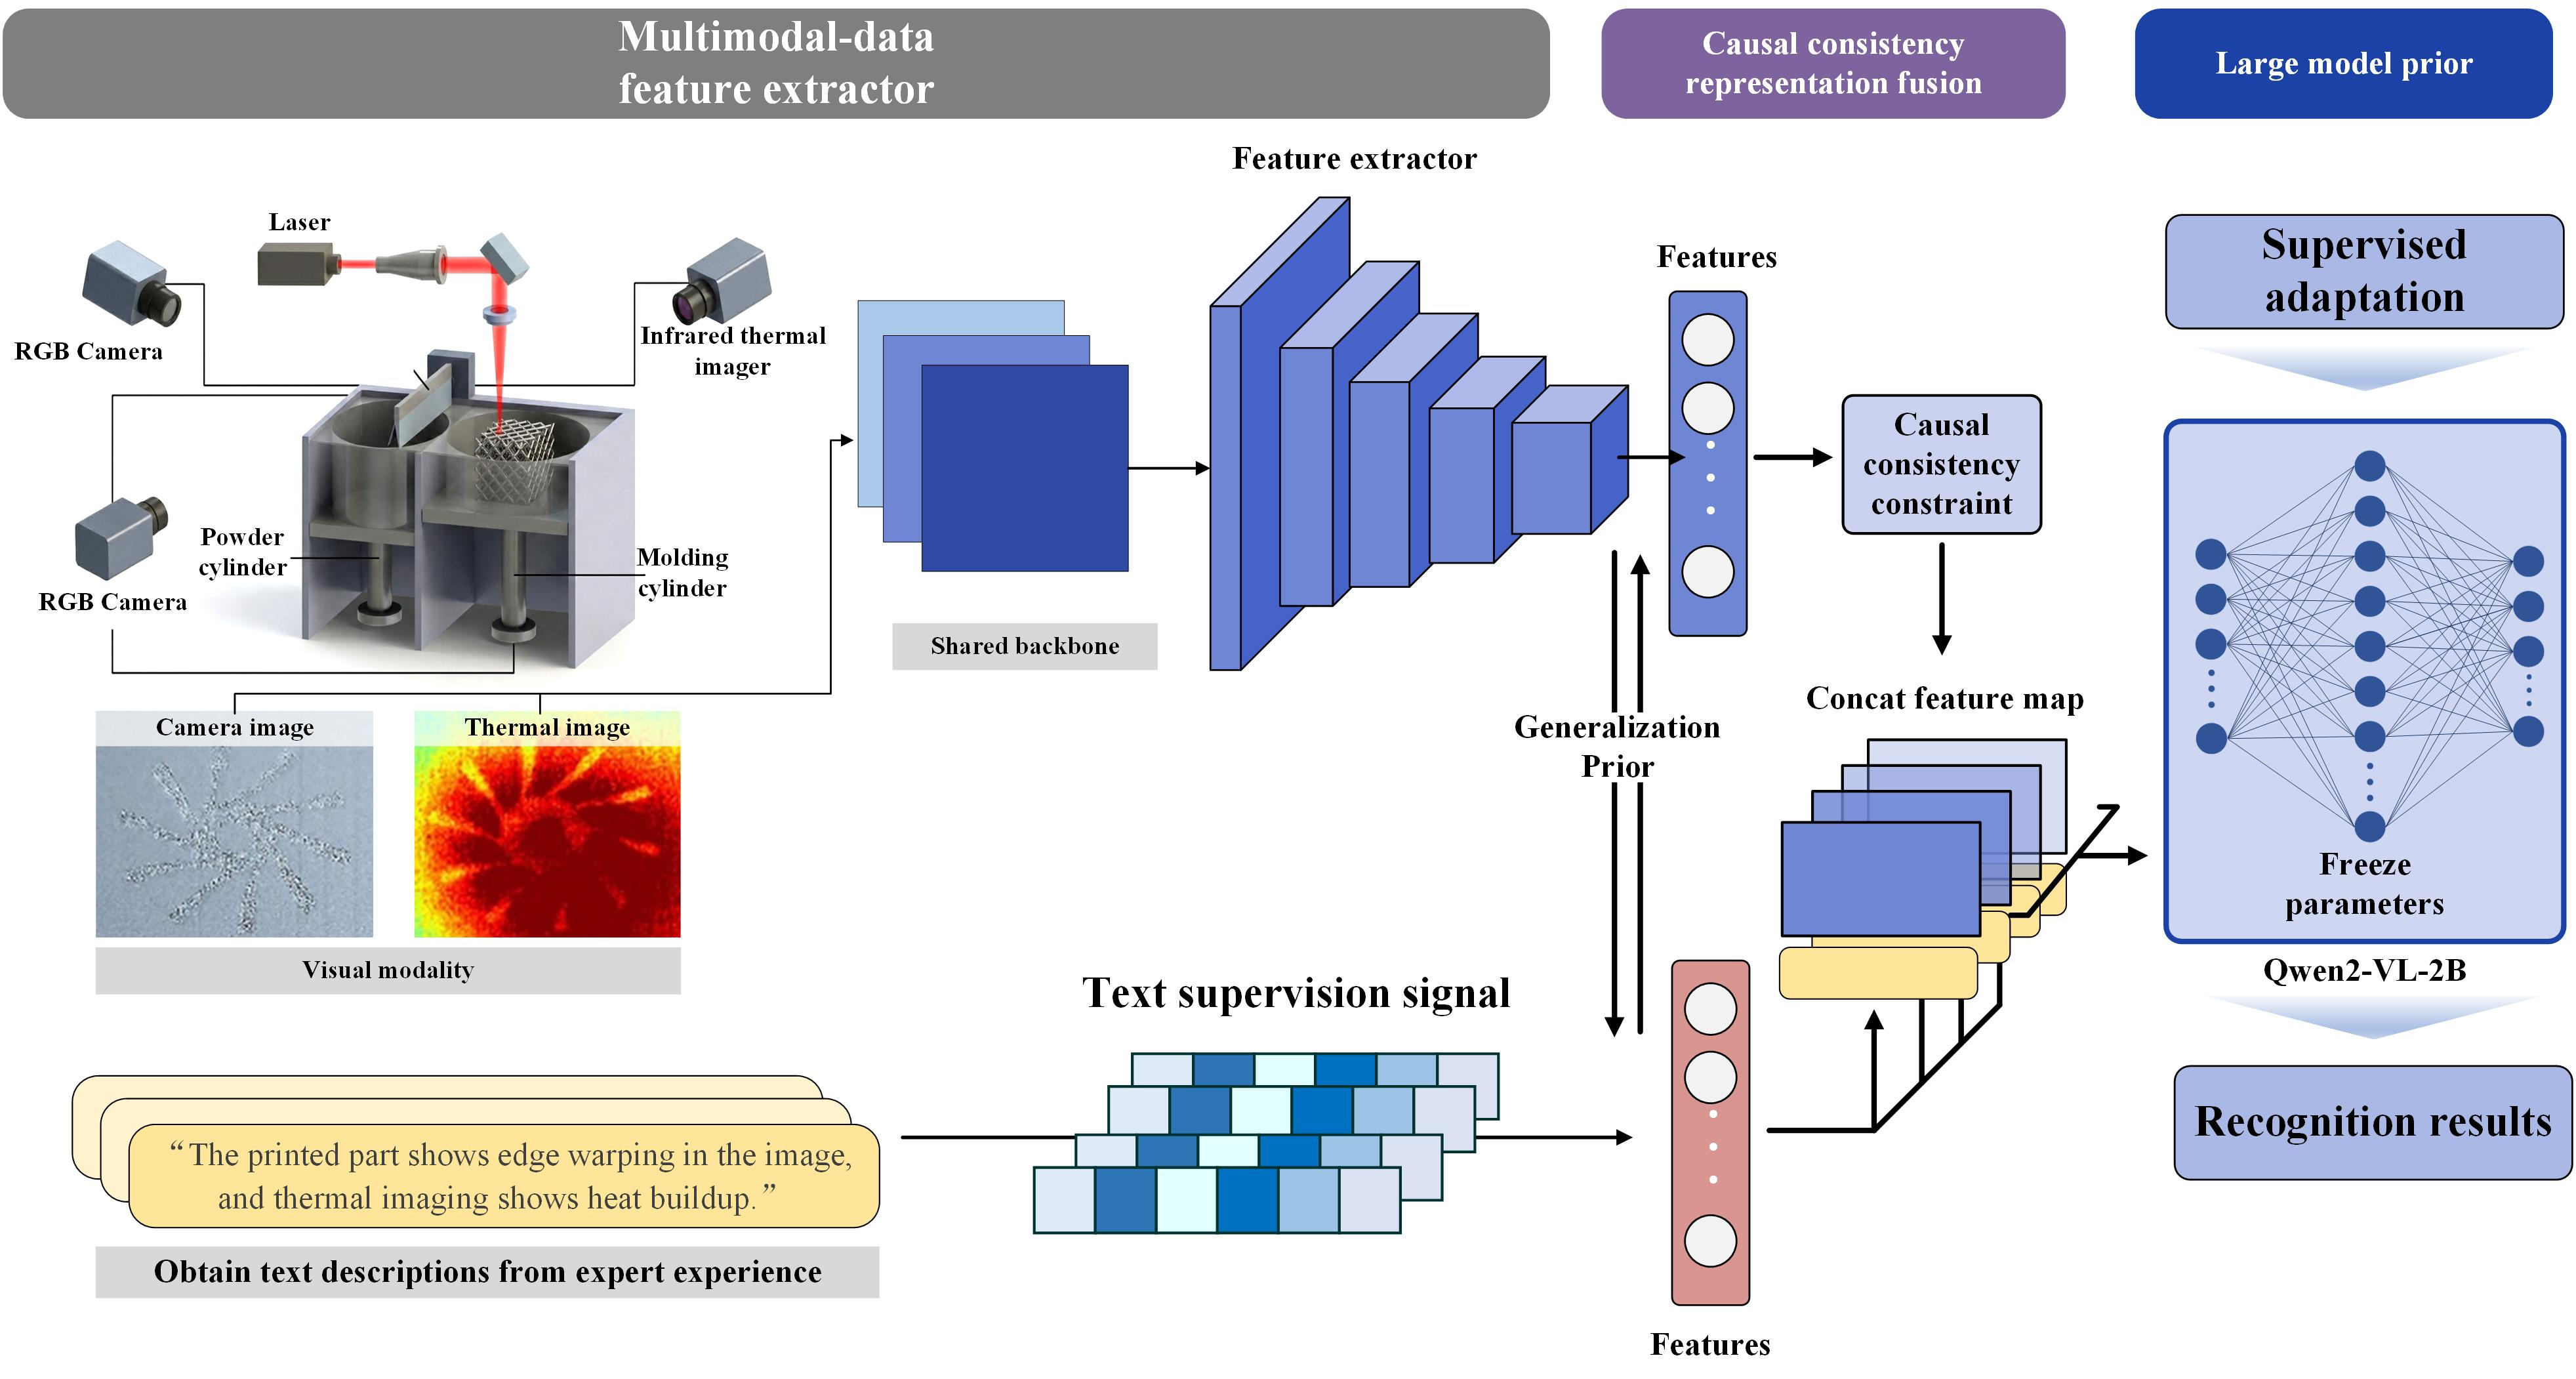
\includegraphics[width=\textwidth]{fig1.jpg}
% \end{graphicalabstract}

%%Research highlights
% \begin{highlights}
% \item Research highlight 1
% \item Research highlight 2
% \end{highlights}

%% Keywords
\begin{keyword}

additive manufacturing\sep multi-modal data fusion\sep anomaly detection.

\end{keyword}

\end{frontmatter}


%% Add \usepackage{lineno} before \begin{document} and uncomment 
%% following line to enable line numbers
%% \linenumbers

%% main text
%%

\section{Nomenclature}

\addcontentsline{toc}{section}{Nomenclature}

{\footnotesize % 缩小表格字体大小
\textcolor{red}{\begin{tabular}{lp{0.68\textwidth}}
\toprule
\textbf{Symbol/Abbreviation} & \textbf{Definition}\\
\midrule
$s_i, s_j$ & Input samples for instances $i$ and $j$ \\
$f(\cdot)$ & Feature extraction function\\
$h_i, h_j$ & Feature vectors of samples $s_i$ and $s_j$\\
$x$ & Input data\\
$y$ & Label of data (healthy-fault)\\
$m$ & Margin parameter for contrastive loss\\
$L_{ctv}$,$L_{cts}$ & Contrastive loss function\\
$L_{CSM}$ & Causal similarity measurement loss\\
$L_{CEMMD}$ & Causal effect maximum mean discrepancy loss\\
$L_{CC}$ & Combined causal consistency loss ($L_{CC}=\alpha L_{CSM}+\beta L_{CEMMD}$)\\
$\alpha,\beta$ & Hyperparameters weighting $L_{CSM}$ and $L_{CEMMD}$\\
$f_e(\cdot)$ & Cross-modal feature extractor\\
$W, b$ & Weights and biases of network layers\\
$\sigma$ & Activation function\\
$z$ & Latent representation vector\\
$Q, K, V$ & Query, key, value matrices (transformer attention)\\
$W_o$ & Weight matrix for multi-head attention output\\
$dk$ & Dimension of transformer keys/values\\
$H$ & Number of attention heads\\
$z_{input}$ & Input features to transformer\\
$z_{fusion}$ & Transformer-based fused features\\
$do(\cdot)$ & Intervention operation (causal inference)\\
$RKHS$ & Reproducing Kernel Hilbert Space\\
$k(\cdot,\cdot)$ & Kernel function\\
\bottomrule
\end{tabular}}
}

\vspace{0.5cm} % 在表格后适当加间距，便于排版

\clearpage

\section{Introduction}

Additive Manufacturing (AM) is a process of creating parts by depositing materials—such as plastics, composites, and metals—layer by layer based on 3D model data, in contrast to traditional formative and subtractive manufacturing methods \cite{RN321}. This technique facilitates the development of complex geometries, shapes, and the customization of material properties to enhance the final product \cite{RN322}. As a result, AM is being increasingly applied across various industries, including automotive, aerospace, aviation, architectural modeling, biomedical engineering, medical/pharmaceutical sectors, and the food industry \cite{RN324}. However, for advanced products, the AM process may be costly and time-consuming. Even small imperfections can lead to significant quality issues, potentially compromising the final product and resulting in substantial economic losses \cite{RN326}. To mitigate these risks, it is crucial to detect and address defects such as porosity, cracking, and geometric distortions early in the manufacturing process.

Deploying monitoring sensors provides real-time information about the AM process, enabling early detection of processing defects and preventing significant losses \cite{RN323}. With continuous research and development, the AM industry now benefits from a broader range of anomaly detection methods enabled by various sensor technologies. For instance, modern AM equipment is frequently equipped with sensors such as acoustic emission (AE), piezoelectric (PE) sensors, accelerometers, gyroscopes, laser scanning devices, or computational vision systems \cite{RN326}. These sensors facilitate the early detection of deviations in the AM process that could lead to defective products. Youssef et al. used optical imaging and infrared (IR) thermography to detect embedded defects in Fused Filament Fabrication (FFF) 3D printing in real-time \cite{RN327}. Mukesh et al. demonstrated the potential of optimizing process parameters, detecting defects, and troubleshooting machine parts using optical, thermal, and acoustic sensors \cite{RN328}. Giulio et al. extracted features from voltage signals through frequency analysis to describe the process state in the Wire Arc Additive Manufacturing (WAAM) process. Several studies have also highlighted the potential for real-time defect detection using accelerometers, gyroscopes, and laser scanning systems \cite{RN329, RN330}. In many AM applications, visual sensors have been effectively deployed to detect defects during the layer-by-layer manufacturing process \cite{RN333}. State-of-the-art in-process monitoring technologies have shown significant potential for defect detection in AM processes. \textcolor{red}{While previous studies have employed multiple sensors, integrating and fusing data from diverse sensor modalities is crucial for capturing the complex interlayer defects that can arise throughout the entire AM process. Relying on individual sensor modalities alone may limit the detection of defects that manifest due to the interaction of multiple factors, such as material flow, temperature variations, and mechanical stresses.} For example, visual monitoring systems may fail to capture clear defect images due to variations in angles and lighting, whereas process-specific parameters may lead to the misinterpretation of normal processes as anomalies by PE/AE sensors \cite{RN325}. Therefore, obtaining more comprehensive information about the manufacturing process is essential for accurate AM anomaly detection.

\textcolor{red}{Integrating information from multiple sensors (multi-modal) provides} a more comprehensive understanding of early defect formation, which is often challenging to capture using a single sensor \cite{RN332}. \textcolor{red}{Fusion of multi-sensor data for anomaly detection has yielded promising results in various applications.} For instance, Alex et al. proposed a multi-modal fusion framework that maps features from point clouds to images, detecting anomalies by identifying inconsistencies between the observed and mapped features \cite{RN334}.\textcolor{red}{Their work laid the groundwork for our approach by demonstrating the effectiveness of multi-modal data fusion in capturing complex sensor data relationships, which we extended to additive manufacturing (AM).} Yue et al. designed an unsupervised feature fusion model to align point cloud and RGB features for anomaly detection in different industrial scenarios \cite{RN335}. Yuanze et al. developed an anomaly detection module based on MiniGPT-4, embedding prior knowledge from vision experts as tokens interpretable by Large Language Models (LLMs) \cite{RN338}. In the context of time series analysis, Mingyu et al. proposed a cross-modal data fusion technique to combine graph data generated by GPS and time-series power output data in renewable energy systems \cite{RN336}. \textcolor{red}{This approach was relevant to our work, as it demonstrated the power of time-series data fusion, which we adapted to combine sensor readings over time in AM processes, such as detecting defects due to variations in temperature or vibration patterns.} Chaoyue et al. introduced a multi-modal spatial-temporal graph attention network (MST-GAT) to model modal correlations for time-series anomaly detection \cite{RN337}. \textcolor{red}{Xinji et al. proposed a multi-modal time series anomaly detection model based on attention autoencoder and generative adversarial network. By integrating distributed control system (DCS) measurement data and acoustic signals, they realized cross-modal feature learning and adversarial regularization optimization in industrial scenarios \cite{ad1}. Chen et al. developed Ano-cDiff, a causal multi-modal diffusion model for brain anomaly detection using counterfactual estimation and adaptive multi-modal data fusion, achieving 8.06\% precision gain in glioma segmentation \cite{ad2}. Their work on causal multi-modal data fusion inspired the integration of causal reasoning into our anomaly detection framework, which improves the interpretability and robustness of the results, particularly when dealing with complex FDM defect detection.}

\textcolor{red}{While these methods have shown promising results in various domains, transformer-based fusion strategies such as those employed in CLIP and MiniGPT-4 are gaining attention in vision-language tasks due to their ability to handle complex multi-modal data \cite{RN338}. However, a key advantage of transformers over traditional attention-based fusion networks lies in their multi-head self-attention mechanism, which enables more effective capture of complex dependencies across modalities. Unlike simpler attention-based fusion networks that rely on basic attention mechanisms, transformers use self-attention to model long-range dependencies between features in different modalities. This allows the model to focus on different parts of the input simultaneously, providing a more comprehensive view of the multi-modal data. In contrast, simpler attention mechanisms in earlier fusion models may focus on only one aspect of the data at a time, which limits their ability to fully capture intricate relationships in complex, multi-modal data. Additionally, transformers can be scaled to handle larger and more diverse datasets, making them particularly well-suited for industrial anomaly detection tasks in dynamic environments, such as additive manufacturing, where data from multiple sensor modalities interact in complex ways.}

\textcolor{red}{Several studies have demonstrated the potential of multi-sensor fusion in additive manufacturing (AM) \cite{RN331}.} For example, Chen et al. developed a spatiotemporal data fusion method that combines acoustic sensors, vision cameras, and laser line scanners for defect detection in AM \cite{RN331}. Kang et al. proposed the Recallable multi-modal data fusion Network (RMFN) to integrate processing, pixel-level, and geometric-level datasets, ensuring consistency of contextual information across sliced layers \cite{RN339}. However, the physical meanings and data modalities of information from cross-modal sensors are fundamentally different—for instance, the sound, vibration, posture, and temperature of the printing process differ significantly from the images of each layer. While current methods have employed artificial intelligence (AI) methods to bridge the differences in feature distributions across multi-modal data \cite{RN341, RN340}, the causal consistency between modalities is often overlooked. As a result, naive AI fusion methods may result in poor performance and an unreliable AM anomaly detection model \cite{RN342}.

In this paper, we propose a framework, illustrated in Fig.\ref{fig1}, termed M3C-AD, for anomaly detection in material extrusion additive manufacturing (AM) through multi-modal-sensor monitoring and reliable feature fusion based on data causality. The key novelty and contribution of this work lie in the development of a novel contrastive causal consistency fusion method based on \textcolor{red}{multi-sensor monitoring data}, which exploits the causal consistency between cross-modal data in the AM process. \textcolor{red}{The sources of data for our multi-sensor fusion include two macro cameras, a three-axis accelerometer, a three-axis vibration sensor, and a temperature sensor.} First, a contrastive feature extraction method is introduced to identify features that are sensitive to anomalies within each sensor modality. Causal consistency alignment is then employed to exploit the causal relationships among cross-modal data, thereby facilitating collaborative learning across multi-sensor data throughout the AM process. Finally, a global coalition fusion layer is used to integrate the aligned multi-modal data. After fusion, the multi-modal feature model can be employed for defect detection and anomaly identification using machine learning techniques.

\begin{figure}[!t]
  \centering
  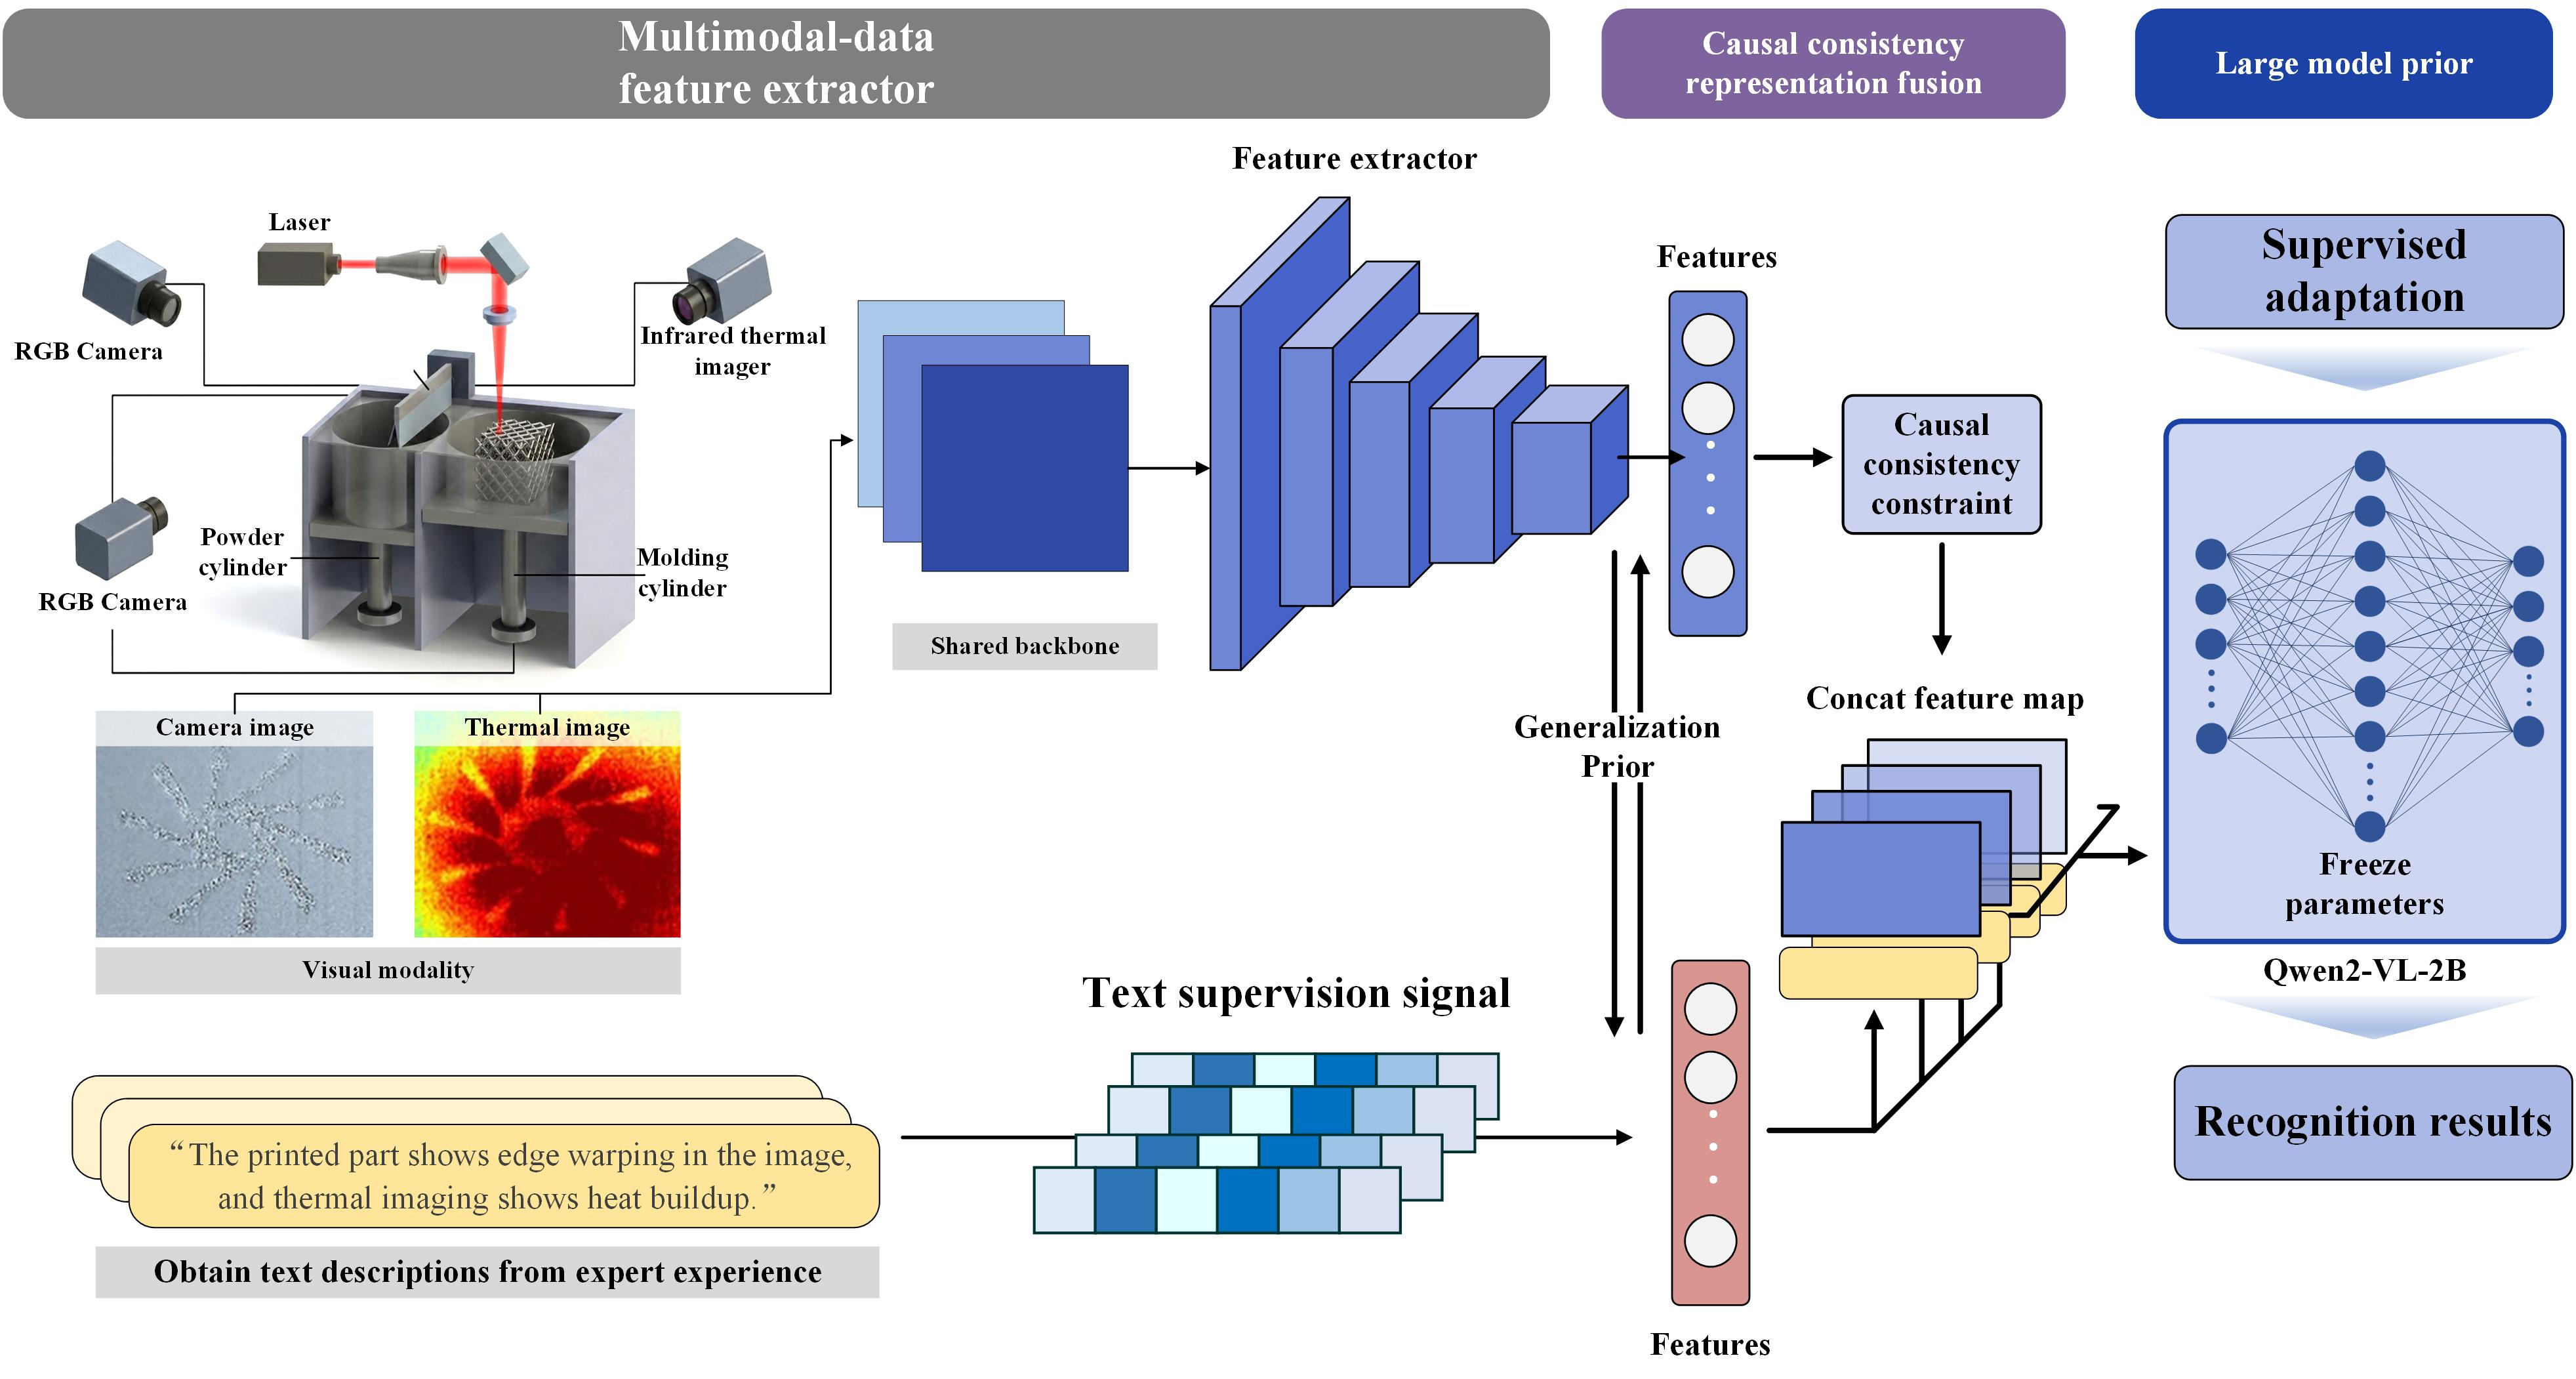
\includegraphics[width=\textwidth]{fig1.jpg}
  \caption{\textcolor{red}{Architecture of the multi-modal contrastive causal consistency fusion anomaly detection (M3C-AD) framework.}}
  \label{fig1}
\end{figure}

In contrast to traditional single-sensor-based monitoring, multi-sensor data fusion enables more reliable and effective anomaly detection for in-situ defect monitoring in additive manufacturing (AM). The proposed contrastive causal consistency fusion method, based on multi-sensor data, addresses the discrepancies between cross-modal data and enhances monitoring reliability by learning the causal consistency among the different data modalities. This framework lays the foundation for self-adaptive AM, offering higher efficiency and accuracy.


\section{Proposed Method}
In this section, we present the multi-modal-sensor feature extraction, contrastive causal consistency alignment, and global collaborative fusion techniques for anomaly detection in additive manufacturing (AM), which represent the main contributions of this work. The proposed multi-modal contrastive causal consistency fusion method lays the foundation for AM process anomaly identification and defect region detection.

\subsection{Local contrastive feature extraction}

\textcolor{red}{Multiple monitoring data are collected from each local sensing modality, as shown in Fig.\ref{fig2}, to provide different perspectives on the additive manufacturing (AM) process. The integration of information from multiple sensor modalities enables the early detection of abnormal conditions, improving the overall reliability of the AM process. Recent studies have explored various sensor monitoring methods for different AM processes, with Table.\ref{tab:sensor_signals} presenting some representative sensor selections. To reflect the real state of the AM process as comprehensively as possible, multi-modal data fusion should integrate monitoring data from a wide range of sensors. However, each sensor modality may exhibit differences in measurement data and redundancy due to variations in their structures, measurement ranges, and principles. These factors must be carefully considered when selecting sensors for fusion. In particular, cost-effectiveness and applicability within the context of the AM process are critical for practical deployment.}

\textcolor{red}{Given that this study focuses on material extrusion-based AM, we prioritize sensors that are not only effective but also economically viable and easy to deploy under the printing bed. Vibration sensors are widely used in this domain because of their cost-effectiveness, stability, and ability to detect subtle early-stage anomalies, such as material defects or process deviations. While force sensors and displacement sensors also have potential applications in AM, they tend to be more costly and are better suited for detecting significant, localized defects rather than early-stage issues. Although this study specifically employs image sensors and vibration sensors, it is important to note that our method has the potential to be extended to other types of sensors. For instance, incorporating thermal sensors or acoustic emission sensors could enhance the system's ability to detect a broader range of anomalies, providing a more robust monitoring solution. The complementarity of multi-modal information significantly enhances the accuracy and robustness of anomaly detection. However, background information across different sensor modalities may be disorganized and may not directly correspond to the anomaly. By applying effective feature extraction techniques, we can better align the target features from different modalities (e.g., workpiece images, vibration signals), thus minimizing fusion errors and improving anomaly detection performance.}



\begin{figure}[!t]
  \centering
  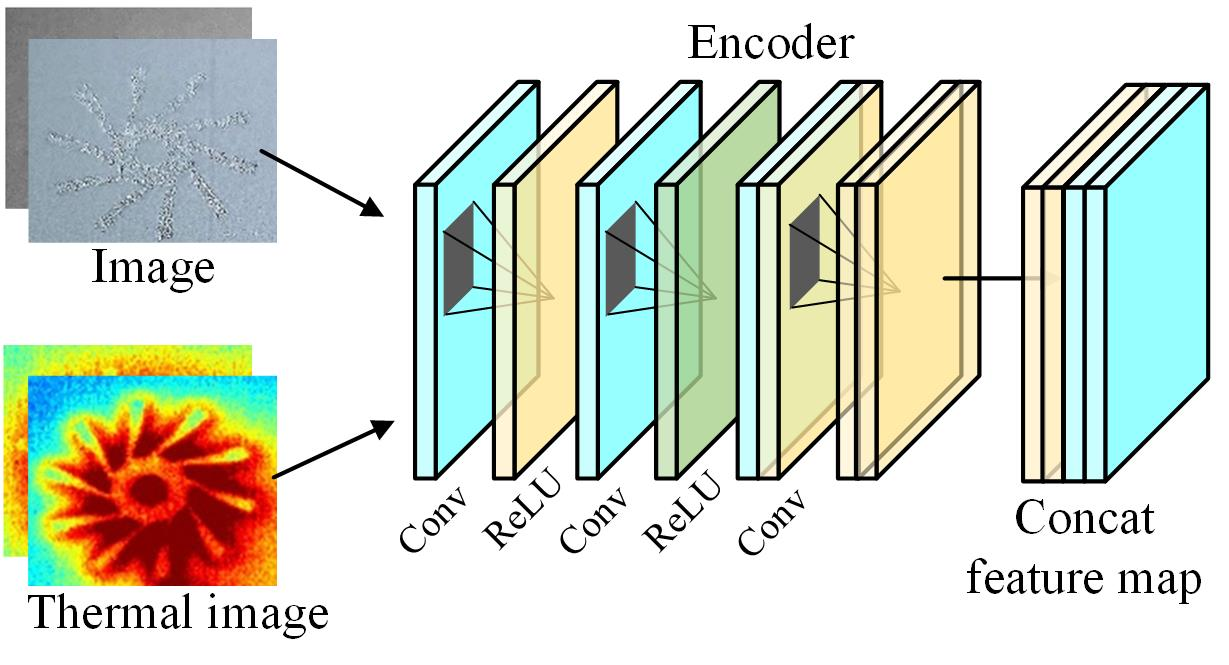
\includegraphics[width=\textwidth]{fig2.jpg}
  \caption{Multi-modal sensor deployment and data collection.}
  \label{fig2}
\end{figure}

\begin{table}[!t]
  \centering
  \caption{\textcolor{red}{Sensor monitoring signals and data modes}}
  \label{tab:sensor_signals}
  \resizebox{\textwidth}{!}{%
  \textcolor{red}{\begin{tabular}{l l l l l l}
  \toprule
  \textbf{Sensor} & \textbf{Monitoring Signal} & \textbf{Data Mode} & \textbf{Sampling Rate} & \textbf{Resolution} & \textbf{Ref.} \\
  \midrule
  Vision       & appearance image, slice image, etc. & 2-D visual image & 30 fps & 1920x1080 pixels & \cite{RN331, RN334, RN323, RN335, RN333} \\
  Thermal      & thermal image & 2-D thermal image & 117 Hz & <25 mK & \cite{RN344} \\
  \midrule
  Acoustic     & acoustic signal & 1-D sequence signal & 30 kHz & $\pm $1.5 dB & \cite{RN331} \\
  Vibration    & vibration signal & 1-D sequence signal & 16 kHz & <F.S$\pm $4\% & \cite{RN346} \\
  Temperature  & temperature signal & 1-D sequence signal & 1 Hz & 0.1°C & \cite{RN347} \\
  Electric     & voltage signal & 1-D sequence signal & 1 kHz & $\pm $0.1 V & \cite{RN345, RN344} \\
  \bottomrule
  \end{tabular}}}
\end{table}

  The complementarity of multi-modal information can significantly enhance the accuracy and robustness of anomaly detection. However, the background information in cross-modal data is often disorganized and may not be directly related to the anomaly. Through effective feature extraction, the target features across different modalities (e.g., workpiece images, fault signals, etc.) can be better aligned, thereby reducing the fusion errors between modalities.

  \subsubsection{2-D Visual image contrastive feature extraction }
  In previous work, many studies have investigated relatively mature visual monitoring systems \cite{RN327, RN328, RN341}. The key challenge in these works lies in the effective extraction of defect area features from the manufactured parts. To address this, and considering the characteristics of the additive manufacturing (AM) process, we designed a contrastive feature extraction layer to assist in subsequent anomaly classification and detection, as shown in Fig.\ref{fig3}. Since the key distinction between healthy and faulty samples is the presence of defects on the AM workpiece, the goal of the feature extractor is to focus the model's feature extraction weights on the workpiece as much as possible. This enables the segmentation of key information from the background, ensuring that subsequent feature fusion is not disrupted by complex background noise. The advantage of using contrastive feature extraction is that by comparing normal and abnormal samples, the model learns to recognize that the core difference lies in the region of the workpiece being processed. This allows the model to focus its feature extraction on the relevant region of the workpiece.

  \begin{figure}[!t]
    \centering
    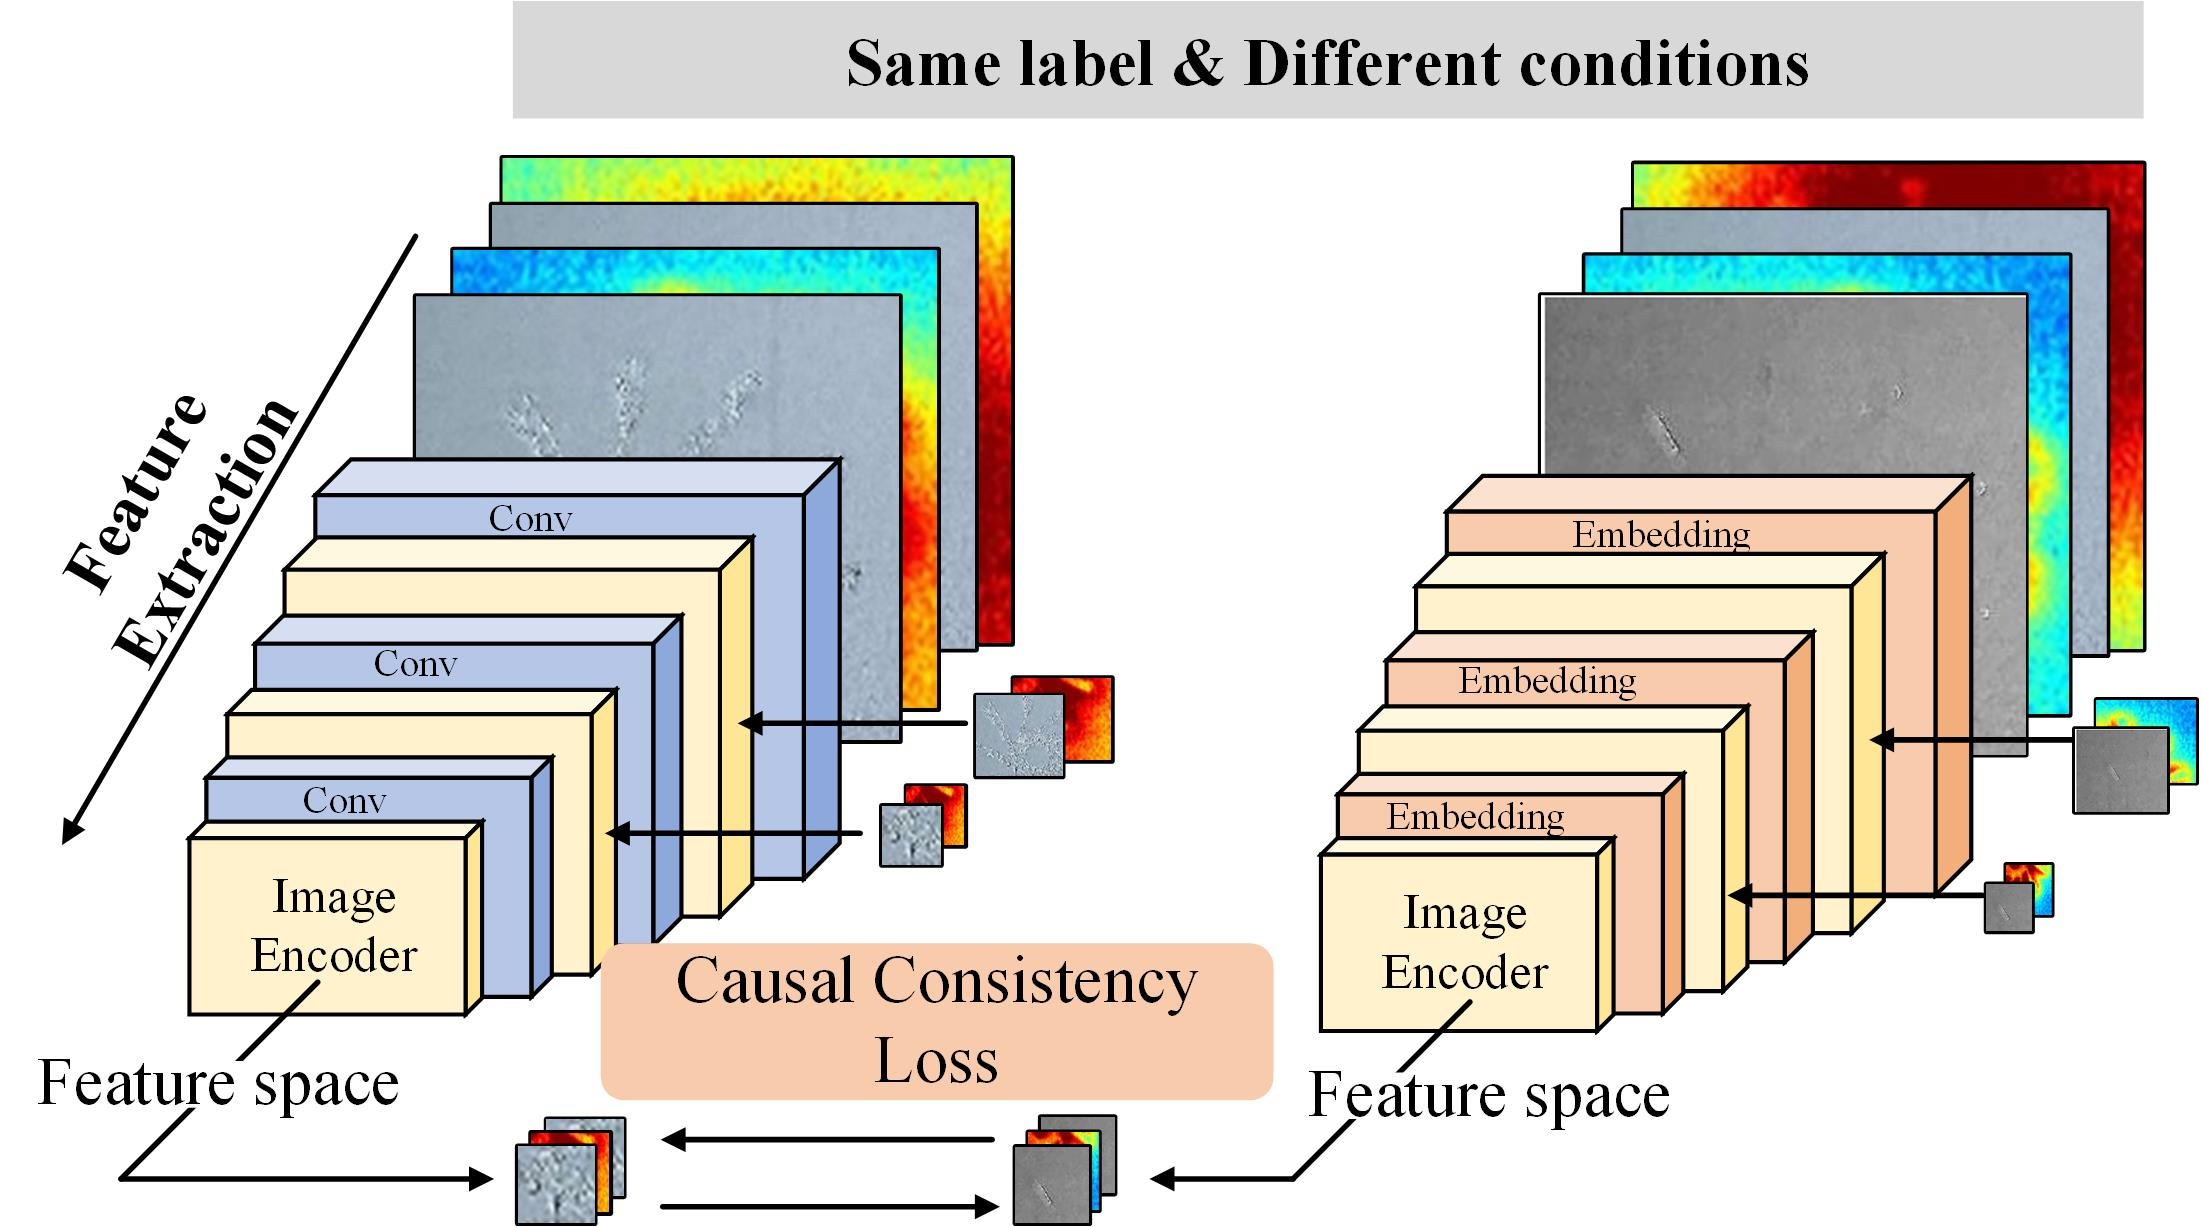
\includegraphics[width=\textwidth]{fig3.jpg}
    \caption{The architecture of the vision contrastive feature extraction layer.}
    \label{fig3}
  \end{figure}

  \textcolor{red}{Define the sample set as $({h}_{i},{h}_{j})$. Positive pairs are defined as those in which both ${h}_{i}$ and ${h}_{j}$ originate from healthy samples of the same modality. Conversely, negative pairs consist of one sample originating from a healthy source and the other originating from a faulty source, both maintained within the same modality. The core idea of contrastive feature extraction is to minimize the distance between positive sample pairs (normal samples) and maximize the distance between negative sample pairs (normal-fault samples), enabling the model to learn the distinguishing features between normal and fault samples. In the context of AM workpiece images, the key distinction between normal and faulty areas lies in the defective region, which can occur anywhere on the workpiece. As a result, the model will focus feature extraction on the workpiece area in the image, thereby ensuring effective extraction of the key features. We achieve a larger distance between normal and faulty sample pairs by constructing the following contrastive loss function:}

  \begin{equation}
    \scalebox{0.9}{$
      \mathcal{L}_{ctv} = (1-y) \cdot \frac{1}{2} \| f(h_i) - f(h_j) \|^2 + y \cdot \frac{1}{2} \max \left( 0, m - \| f(h_i) - f(h_j) \| \right)^2
    $.}
    \label{eq1}
  \end{equation}

  \textcolor{red}{Let$f(\cdot)$ represent the output of the feature extraction network (e.g., a convolutional neural network), and let $y$ denote the label indicating normal/fault sample pairs. Note that in $f(\cdot)$, the symbol $\cdot$ serves merely as a placeholder for the input argument (e.g., $f(h_i)$ denotes the feature vector extracted from sample $h_i$) and does not indicate a dot product. The features $h_i$ and $h_j$ correspond to data-derived representations. Here, $y=0$ indicates that both $h_i$ and $h_j$ belong to the healthy class (positive pair), while $y=1$ signifies pairs containing one healthy and one faulty sample (negative pair). The hyperparameter $m>0$ enforces a separation margin between healthy and faulty embeddings. Post-training, the feature extraction component of the contrastive learning model facilitates focused key feature extraction, as the optimized model prioritizes learning discriminative patterns in critical workpiece regions.}

  \subsubsection{1-D Vibration signal contrastive feature extraction}

  In the context of additive manufacturing (AM), vibration signals are often used to monitor the displacement and frequency of the workpiece. Deploying vision-based monitoring solutions allows for clear observation of the morphology of abnormal areas, but it is often difficult to detect early weak abnormal features. Vibration-based monitoring methods offer distinct advantages, such as the ability to capture weak abnormal vibration signals as soon as they occur. While vibration signals are less intuitive than visual signals, they are widely deployed in various industrial applications due to their advantages, including sensitive response, rapid deployment, and low cost. However, due to the complex mechanical movements and interference between different systems in the AM process, key sequence signals are often coupled with noise, causing abnormal features to be submerged in these background noise fragments. To address this, we designed a contrastive feature extraction layer for vibration signals to assist in subsequent anomaly classification and detection, as shown in Fig.\ref{fig4}. The goal of the feature extractor is to focus the model's feature extraction weights on the fault signal as much as possible, enabling the model to extract the key information from the vibration signal. The advantage of using contrastive feature extraction is that by comparing normal and abnormal samples, the model learns to recognize that the core difference lies in the fault signal. This allows the model to focus its feature extraction on the relevant region of the vibration signal.


  \begin{figure}[!t]
    \centering
    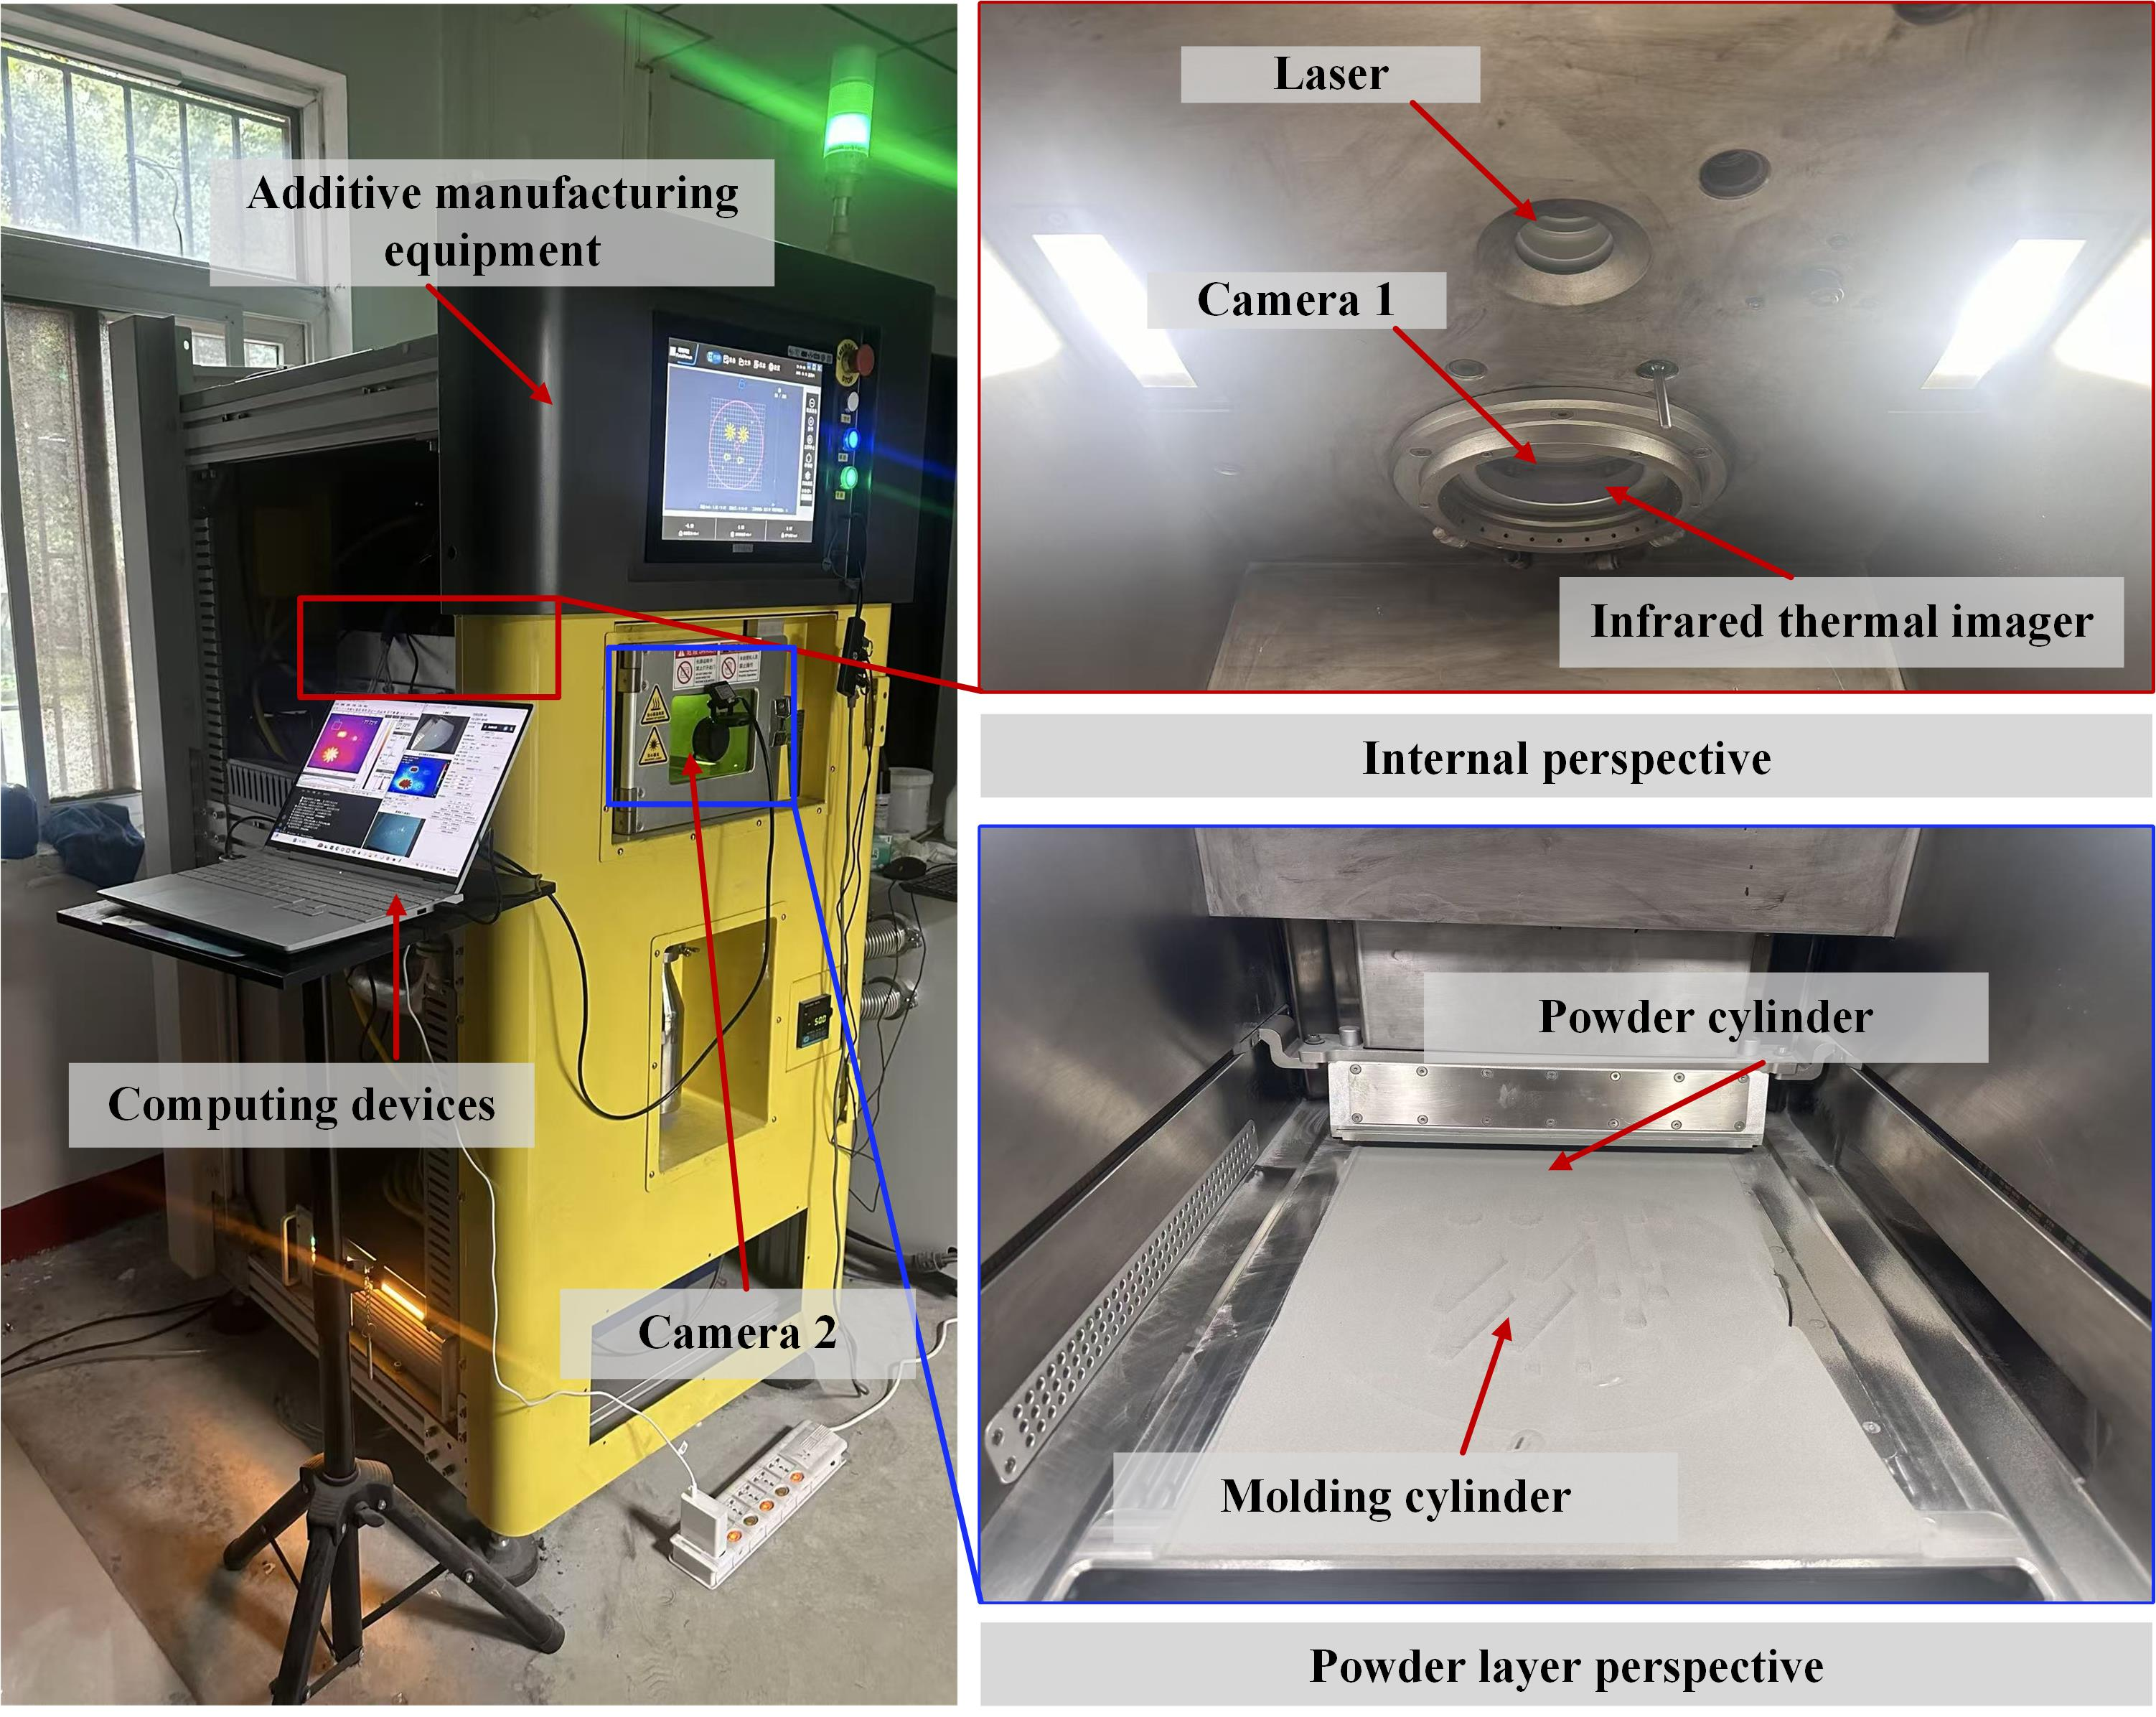
\includegraphics[width=\textwidth]{fig4.jpg}
    \caption{The architecture of the sequence signal contrastive feature extraction layer.}
    \label{fig4}
  \end{figure}

  \textcolor{red}{Define the sample set as $(s_i, s_j)$, where a positive pair consists of two healthy samples from the same modality and a negative pair comprises one healthy sample and one fault sample. The key objective of contrastive feature extraction is to pull together the features of positive pairs while pushing apart those of negative pairs, thereby enabling the model to learn discriminative representations for normal and fault samples. To enforce this, we design the following loss function:}

  \begin{equation}
    \scalebox{0.9}{$
      \mathcal{L}_{cts} = (1-y) \cdot \frac{1}{2} \| f(s_i) - f(s_j) \|^2 + y \cdot \frac{1}{2} \max \left( 0, m - \| f(s_i) - f(s_j) \| \right)^2
    $.}
    \label{eq2}
  \end{equation}

Let $f(\centerdot )$ represent the output of the feature extraction network (such as a convolutional neural network), and let $y$  denote the label of the normal-fault samples. After training, the feature extraction component of the contrastive learning model can be used for initial key feature extraction.


\subsection{Causal consistency alignment}

\subsubsection{\textcolor{red}{Causal consistency in multi-modal data}}

\textcolor{red}{Abnormalities in the additive manufacturing process should be caused by their root faults, such as improper process parameters, incidental factors in processing, and failures of the equipment itself \cite{RN342}. Anomalies caused by these potential factors will exhibit different anomaly features on the data recorded by different sensors. But even if the anomalies are characterized differently on different modalities of the data, the root causes of their failures should be the same, i.e., there exists a causally consistent features of their failure characteristics. Formally, for each modality $M_i$, its observed data $X_i$ should satisfy the condition: }

\textcolor{red}{\begin{equation}
P(X_i|\text{Pa}(X_i))=P(X_i|\{X_j:M_j\in\text{Pa}(M_i)\})
\label{eq_ad1}
\end{equation}}
\textcolor{red}{where $\text{Pa}(M_i)$ denotes the set of modalities that have a causal influence on $M_i$.  Causal consistency implies that the inferred or learned data distributions across modalities maintain alignment with these dependencies, ensuring coherent multi-modal reasoning. The causal relationship between different modalities of data is consistent, and the root cause of the anomaly is consistent across multi-modal data. The core of causal consistency alignment is to ensure that the causal relationship between these modal data is properly modeled and aligned.}

\textcolor{red}{As illustrated in Fig. \ref{fig5}, the abnormal causal consistency representation between the feature distributions of different modalities implies that, even if the observed data of the abnormal state differ across modalities, their inherent causal relationship remains consistent\cite{RN256}.}

\begin{figure}[!t]
  \centering
  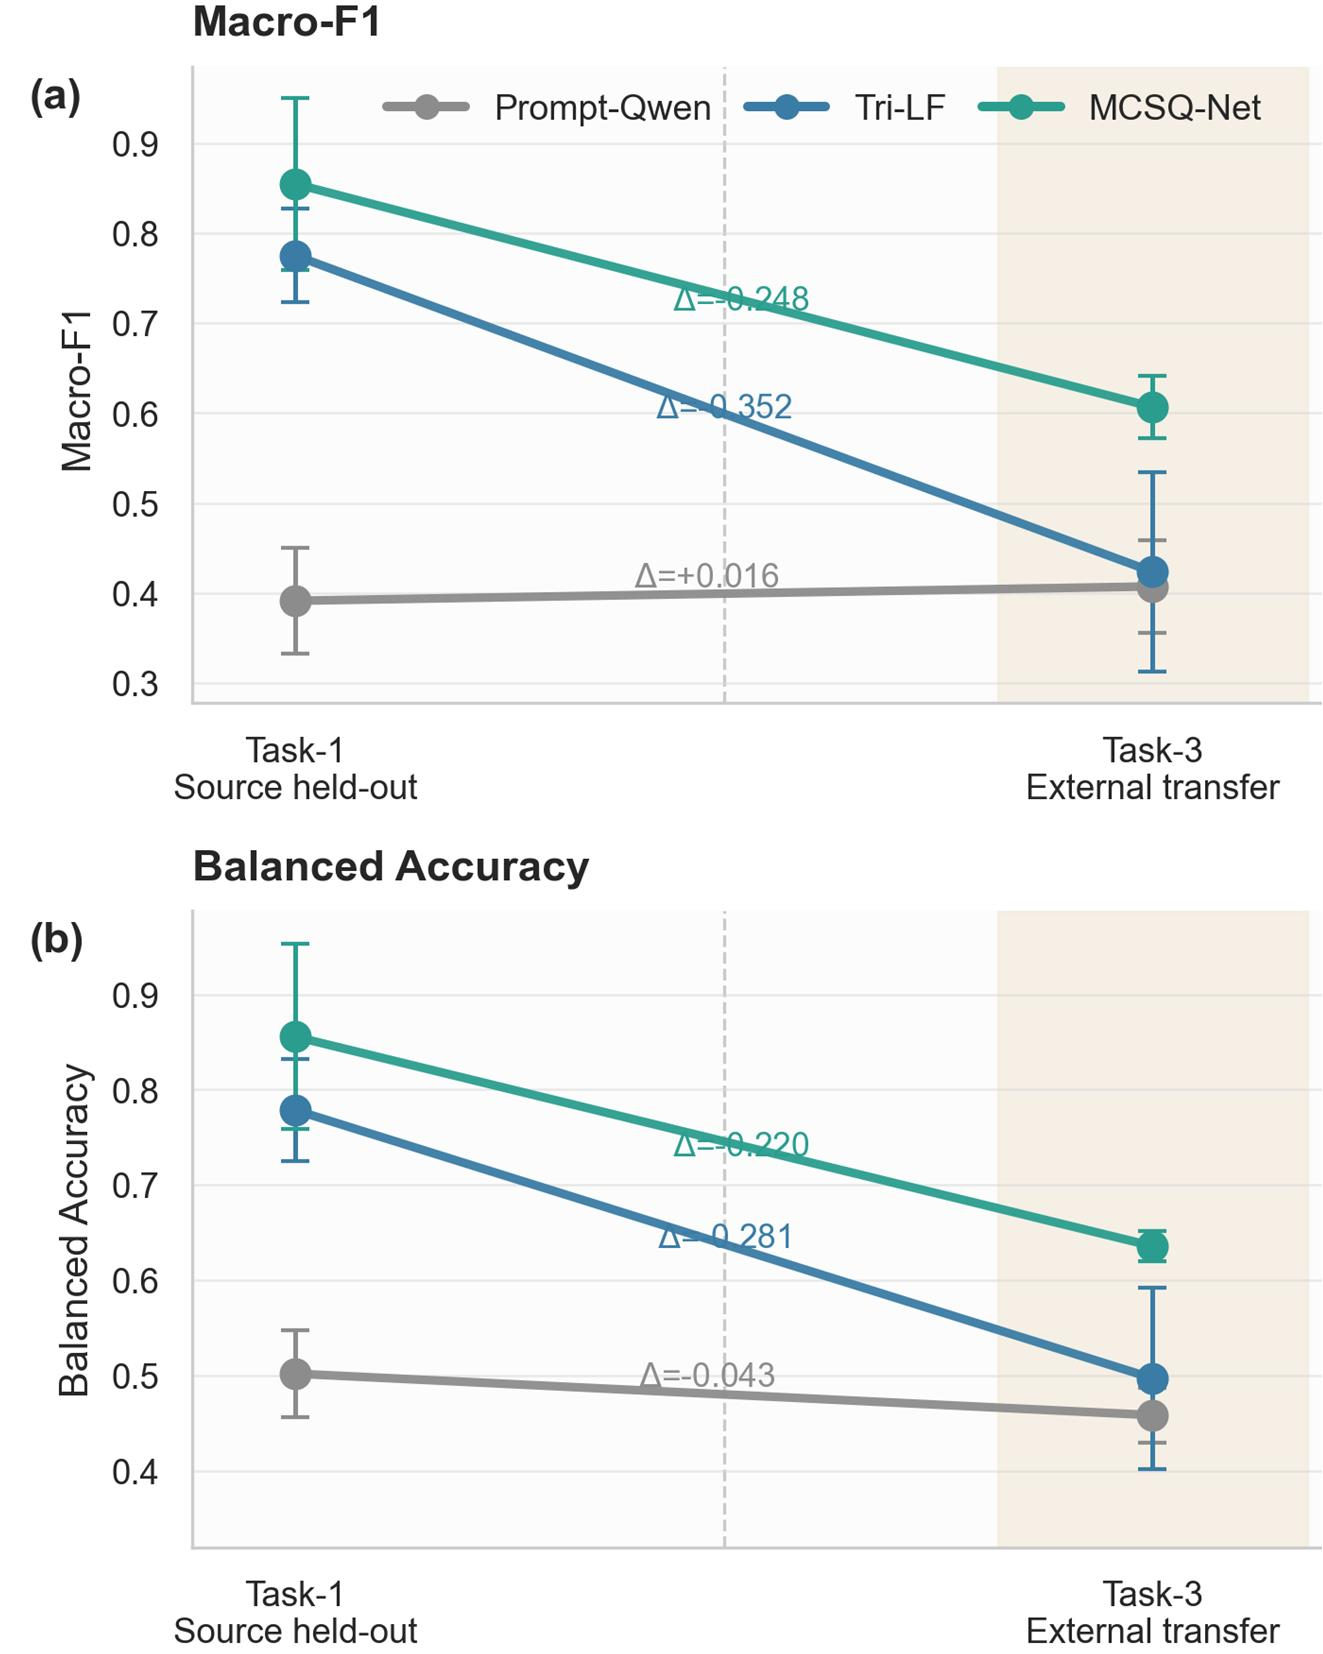
\includegraphics[width=\textwidth]{fig5.jpg}
  \caption{The root cause of the anomaly is consistent across multi-modal data, resulting in a causal consistency representation of the abnormal state, which can be mined by using causal similarity measurement (CSM) and causal effect maximum mean discrepancy (CEMMD).}
  \label{fig5}
\end{figure}


\subsubsection{\textcolor{red}{Causal consistency loss}}

In order to mine the anomalously causal consistent features of different modal monitoring data, define a cross-modal feature extractor ${{f}_{e}}(\centerdot )$ that can learn the observational data $x$ as follows:

\begin{equation}
  \scalebox{0.9}{$
    z={{f}_{e}}(x)=\sigma (Wx+b)$}.
  \label{eq3}
\end{equation}
where $x\in {{\mathbb{R}}^{n}}$, $W\in {{R}^{k\times n}}$ is the weight matrix of ${{f}_{e}}(\centerdot )$, $\sigma $ is the activation function, and $b\in {{R}^{k}}$ is the bias term. The latent representation $z\in {{\mathbb{R}}^{k}}$ obtained from the encoder ${{f}_{e}}(\centerdot )$ is the characteristic representation of the observable data in a low-dimensional space.

For faulty data in multi-modal systems, the anomaly state exhibits a positive correlation with changes in the process monitoring signals, which include both image and sequence signals. For example, when a defect occurs in the workpiece, it will be visible in the image, and an abnormal vibration signal will be generated. The occurrence of these abnormal signals is synchronous, meaning that the cross-modal feature extractor will focus on these features in a similar manner during training \cite{RN343}. Therefore, we infer that if the multi-modal feature extractor ${{f}_{e}}(\centerdot )$ is learning causal consistent features, the model's learning behavior will tend to be consistent. The objective function for causal features ${{Z}_{c}}$ can then be defined as:

\begin{equation}
  \scalebox{0.9}{$
    Z={{Z}_{c}}\Rightarrow \arg \max g[{{f}_{e}}({{X}_{1}}),{{f}_{e}}({{X}_{2}})]$}.
  \label{eq4}
\end{equation}
where the data ${{X}_{i}}$ from the multi-modal dataset ${{X}_{\text{multi-modal}}}=\{{{X}_{i}}|i=1,\cdots ,m\}$, and $g(\centerdot )$ is the causal similarity measurement function (CSM). Based on cosine similarity to estimate the consistency of the cross-modal extractor, ${{\mathcal{L}}_{CSM}}$ can be written as:

\begin{equation}
  {{\mathcal{L}}_{CSM}}=1-abs(\frac{({{W}_{1}}{{x}_{1}}+{{b}_{1}})\centerdot ({{W}_{2}}{{x}_{2}}+{{b}_{2}})}{\left\| ({{W}_{1}}{{x}_{1}}+{{b}_{1}}) \right\|\left\| ({{W}_{2}}{{x}_{2}}+{{b}_{2}}) \right\|}).
  \label{eq5}
\end{equation}

The smaller the ${{\mathcal{L}}_{CSM}}$ value, the more consistent the feature extractor's learning behavior is across different modalities.

For causal effect estimation, since the causal mechanism between different modalities is consistent, the changes in causal effects should also be consistent. In causal inference, intervention analysis is commonly used to estimate causal effects. Here, $do(X=x)$ represents an intervention on $X$ to observe its effect on $Y$. The formula for the causal effect expectation is as follows:

\begin{equation}
  \scalebox{0.9}{$
  E[Y\mid do(X=x)]=\int P(Y\mid X=x,Z=z)P(Z=z)dz$}.
  \label{eq6}
\end{equation}

Here, $Z$ is the control variable in the latent space, and $P(Y\mid X=x,Z=z)$ represents the conditional probability. Since the root causes (i.e., causal features ${{Z}_{c}}$) of fault signals in different modalities are the same, the objective function for causal effect estimation under ideal causal characteristics should be:

\begin{equation}
  \scalebox{0.9}{$
  Z={{Z}_{c}}\Rightarrow \arg \min ||E[{{Y}_{1}}\mid do({{X}_{1}})]-E[{{Y}_{2}}\mid do({{X}_{2}})]||$}.
  \label{eq7}
\end{equation}

Introducing the reproducing kernel function $\phi (\centerdot )$ to map the distribution of different modal data ${{X}_{i}}$ into a high-dimensional Reproducing Kernel Hilbert Space (RKHS), we can define the causal effect maximum mean discrepancy (CEMMD) as:

\begin{equation}
  \scalebox{0.9}{$
  CEMM{{D}^{2}}=\|{{\mathbb{E}}_{Y\sim P(Y|do({{X}_{1}}))}}[\phi ({{Y}_{1}})]-{{\mathbb{E}}_{Y\sim P(Y|do({{X}_{2}}))}}[\phi ({{Y}_{2}})]\|_{\mathcal{H}}^{2}$}.
  \label{eq8}
\end{equation}

Since $Y={{f}_{cls}}(Z)$, where ${{z}_{i}}\in {{Z}_{i}}$ represents the latent features of different modalities, the causal effect maximum mean discrepancy (${{\mathcal{L}}_{CEMMD}}$) can be approximately estimated as:

\begin{equation}
  \scalebox{0.9}{$
  {{\mathcal{L}}_{CEMMD}}=\frac{1}{{{m}^{2}}}\underset{i=1}{\overset{m}{\mathop \sum }}\,\underset{j=1}{\overset{m}{\mathop \sum }}\,k({{z}_{1}},{{z}_{1}})+\frac{1}{{{n}^{2}}}\underset{i=1}{\overset{n}{\mathop \sum }}\,\underset{j=1}{\overset{n}{\mathop \sum }}\,k({{z}_{1}},{{z}_{2}})-\frac{2}{mn}\underset{i=1}{\overset{m}{\mathop \sum }}\,\underset{j=1}{\overset{n}{\mathop \sum }}\,k({{z}_{1}},{{z}_{2}})$}.
  \label{eq9}
\end{equation}

The smaller the value of CEMMD, the more consistent the causal learning effect of the feature extractor is across different modal data. Finally, we can use the above formula to compute the loss function of the causal consistency representation in the multi-modal feature extraction phase as follows:

\begin{equation}
  \scalebox{0.9}{$
  {{\mathcal{L}}_{CC}}=\alpha {{\mathcal{L}}_{CSM}}+\beta {{\mathcal{L}}_{CEMMD}}$}.
  \label{eq10}
\end{equation}

Here, $\alpha$ and $\beta$ are hyperparameters, which are determined through the actual training optimization process.

\subsection{Global collaborative fusion}

After the causal mechanisms between multiple modalities are consistently aligned, the learning behavior of the network and the feature space distributions of different modalities exhibit consistency. This consistency is reflected by minimizing the loss in the causal consistency objective function above. The features $Z$ of each modality are projected into the same feature space for fusion. Linear projection functions $l(\centerdot )$ can be used to achieve the alignment of different feature sets $Z$ as:

\begin{equation}
  \scalebox{0.9}{$
  \left\{ \begin{matrix}
    {{V}_{1}}={{l}_{1}}({{Z}_{1}})  \\
    {{V}_{2}}={{l}_{2}}({{Z}_{2}})  \\
 \end{matrix} \right.
 $}.
  \label{eq11}
\end{equation}

Where ${{V}_{1}}$ and ${{V}_{2}}$ represent the feature representation vectors projected into the same feature space. Traditional feature fusion methods typically concatenate and fuse features in the same feature space to obtain a higher-dimensional multi-modal feature vector. However, this method can lead to the loss of modality-specific characteristics, as some modalities may possess more significant capabilities in representing abnormalities. Several studies have used machine learning algorithms, such as attention mechanisms or MLPs, to achieve feature fusion with successful results \cite{RN334, RN335}. \textcolor{red}{Building on this prior work, we introduce an advanced transformer architecture to achieve high-dimensional feature fusion, as shown in Fig.\ref{fig6} and Table.\ref{tab:transformer_architecture}. The advantage of this method lies in its use of the global attention mechanism, which enables the optimal allocation of learning weights for different modal features \cite{RN348}. We define the attention weight matrix as:}

\begin{table}[!t]
  \centering
  \caption{\textcolor{red}{Multi-modal data fusion layer architecture}}
  \label{tab:transformer_architecture}
  \textcolor{red}{
  \begin{tabular}{ll}
  \toprule
  \textbf{Component} & \textbf{Specification} \\
  \midrule
  Transformer Layers & 2 \\
  Attention Heads per Layer & 4 \\
  Embedding Dimension & 256 \\
  Attention Mechanism & Multi-head Self-Attention \\
  Input Tokens & multi-modal specific features \\
  Feedforward Network (FFN) & Hidden size = 512 \\
  Positional Encoding & Learnable positional embeddings \\
  Fusion Strategy & Multi-modal global attention\\
  Output Aggregation & Average pooling over token outputs \\
  \bottomrule
  \end{tabular}}
  \end{table}

\begin{figure}[!t]
  \centering
  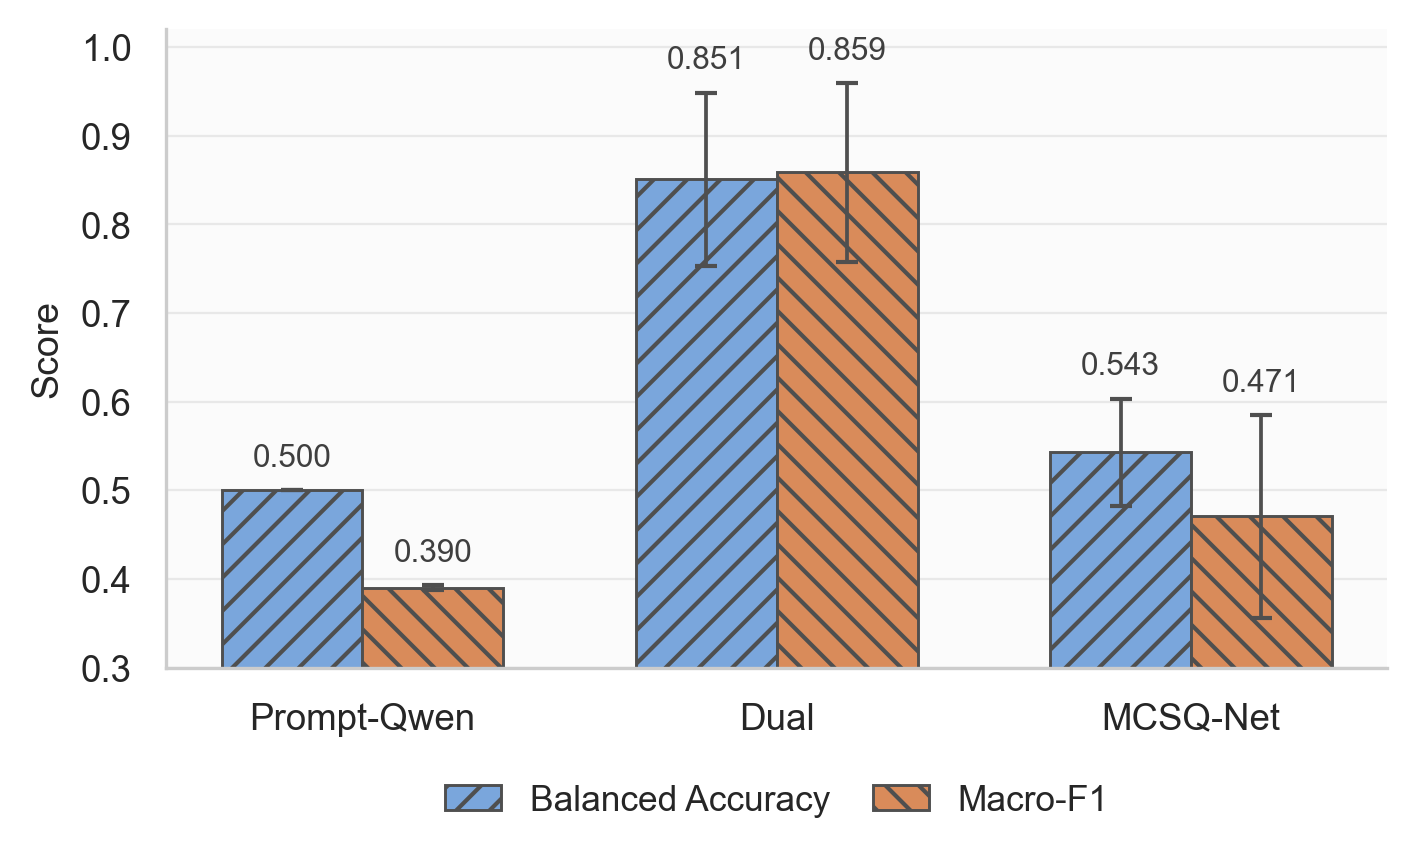
\includegraphics[width=\textwidth]{fig6.jpg}
  \caption{The architecture of the global collaborative fusion layer.}
  \label{fig6}
\end{figure}

\begin{equation}
  \scalebox{0.9}{$
  \text{Attention}(Q,K,V)=softmax\left( \frac{Q{{K}^{T}}}{\sqrt{{{d}_{k}}}} \right)V
 $}.
  \label{eq12}
\end{equation}

Where $Q$, $K$, $V$ represent the queries, keys, and values derived from  ${{V}_{1}}$ and ${{V}_{2}}$, ${{d}_{k}}$ denotes the dimension of the key and value. The expression for the multi-head attention mechanism is:

\begin{equation}
  \scalebox{0.8}{$
  \text{MultiHead}(Q,K,V)=\text{Concat}(softmax\left( \frac{{{Q}_{1}}{{K}_{1}}^{T}}{\sqrt{{{d}_{k}}}} \right){{V}_{1}},\cdots ,softmax\left( \frac{{{Q}_{i}}{{K}_{i}}^{T}}{\sqrt{{{d}_{k}}}} \right){{V}_{i}}){{W}_{o}}
 $}.
  \label{eq13}
\end{equation}

Where ${{W}_{o}}\in {{\mathbb{R}}^{H{{d}_{k}}\times d}}$ is the parameter matrix for the linear transformation, and $H$ represents the number of attention heads. The output of each self-attention layer passes through residual connections and layer normalization to stabilize training and preserve the original information, as shown below:

\begin{equation}
  \scalebox{0.8}{$
  {{z}_{fusion}}=\text{LayerNorm}(\text{MultiHead}({{z}_{input}})+{{z}_{input}})
 $}.
  \label{eq14}
\end{equation}

Where ${{z}_{input}}$ represents the $Q$, $K$, $V$ of the features from each modality. At this point, we have obtained the fused features ${{z}_{fusion}}$, in which the specificity of each modality is preserved through the multi-head self-attention mechanism of the transformer module, ensuring strong performance in downstream tasks such as anomaly classification and anomaly detection. 



\section{Experiment}


\subsection{\textcolor{red}{Experiments platform setup}}

\textcolor{red}{A Creality Ender 3-S1 FDM printer was constructed and integrated with a manufacturing process monitoring and anomaly detection system for this study. As shown in Fig.\ref{fig7}, this printer primarily provides two modalities of monitoring data: 2D image data of the additive manufacturing (AM) process captured by a camera, and vibration, acceleration, and temperature data obtained from a 9-axis vibration sensor. For the 2D image acquisition, we tested the performance of various cameras and lenses, including the Canon R50 with an 18-45mm lens, the Nikon Z30 with a 16-50mm lens, the Sony a7c2 with an 18-66mm lens, and the USB webcam Logitech C270. After comparison, it was found that as long as the camera can clearly capture the quality of the manufacturing process and is easy to deploy, the specific camera model had little impact on the results. Consequently, the low-cost consumer-grade camera, the Logitech C270, was selected for the experiment. While image-based monitoring is effective in localizing visible defects, it suffers from a critical limitation: anomalies are typically detected only after defects have become apparent, by which point it is often too late for intervention. To address this limitation, our system also incorporates a 9-axis vibration sensor for 1D signal acquisition. The Wit-motion WTVB02-485 sensor is used to collect 3-axis acceleration, 3-axis vibration displacement, and 3-axis vibration frequency data, which offer complementary insights into process dynamics and enable earlier detection of potential faults.}



\begin{figure}[!t]
  \centering
  \includegraphics[width=\textwidth]{fig7.jpg}
  \caption{The experimental platform setup based on the Creality Ender 3-S1 FDM printer.}
  \label{fig7}
\end{figure}

\subsection{\textcolor{red}{Data collection and preprocessing}}

Parts produced by additive manufacturing (AM) are increasingly being utilized in the aerospace industry. Non-metallic materials, in particular, play a crucial role in civil aircraft manufacturing due to their ability to significantly reduce weight while maintaining structural integrity and complexity. For instance, the Airbus A350 XWB uses low-pressure air ducts made from ULTEM 9085 material, produced using FDM technology by Stratasys \cite{RN355}. In our experiments, we selected the low-pressure air duct connector model as a case study for anomaly detection. To simplify the experiment, PLA material was used to simulate the manufacturing process, and the model was simplified to facilitate testing. Using the multiple sensors deployed as described earlier, we collected specific data.

  In terms of data processing, to facilitate comparison with existing image anomaly detection methods, we normalized and cropped the images to a fixed size of insert pixel size, with mean values of (0.485, 0.456, 0.406) and variances of (0.229, 0.224, 0.225). For the sequence signal data, in order to align the feature information with the image modality, we applied sliding window segmentation in addition to standard normalization. As shown in Fig.\ref{fig8}, each segment of the signal corresponds one-to-one with the time of image capture. Specifically, we extracted 114 data points before and after the image capture, totaling 224 points for each sequence signal sample.

  \begin{figure}[!t]
    \centering
    \includegraphics[width=\textwidth]{fig8.jpg}
    \caption{Sliding window segmentation of sequence signal data in	multi-modal data.}
    \label{fig8}
  \end{figure}


\subsection{\textcolor{red}{Data set description}}
The dataset for our multi-modal fusion approach consists primarily of image data from both axes and various sensor data, including acceleration, vibration displacement, and vibration frequency, collected by vibration sensors.

For the image data, as shown in Fig.\ref{fig9}(a), images captured from both axes are categorized into three materials and colors, containing both normal and abnormal X and Y observation angle images.

For the vibration signal data, the time-domain waveform is illustrated in Fig.\ref{fig9}(b). The vibration signals include 3-axis acceleration, 3-axis vibration displacement, and 3-axis vibration frequency. The data is stored in CSV format, with 224 data points selected as a single sample for model training, based on the specific time points of their recording, to align with the image timestamps for fusion.

\textcolor{red}{In the dataset, the defects on the workpiece mainly include warping, porosity, and cracking. The root cause of these defects is the blockage of the print head (artificial intervention). Since the anomaly detection task mainly focuses on detecting anomalies without specifically distinguishing the types of anomalies, we uniformly mark these defect forms as anomalies. For example, common printing faults observed in our setup include warping of the part (portions lifting or curling due to uneven cooling or poor bed adhesion) and stringing (thin filament strands between features caused by nozzle oozing during travel moves). We also encountered layer cracking or breakage, often triggered by extruder head clogs that result in insufficient material deposition. Each of these faults is visibly evident in the print and corresponds to distinct signatures in the sensor data. The dataset comprises 5,040 samples (Normal samples: 3033, Anomalous samples: 2007), where each sample corresponds to a print moment with synchronized multi-modal time-series data and image data.}

\begin{table}[!t]
  \centering
  \caption{\textcolor{red}{Data modalities and associated information}}  % 表格标题放在表格前
  \resizebox{\textwidth}{!}{  % 将表格宽度调整为文本宽度
  \textcolor{red}{
  \begin{tabular}{ccccc}
  \toprule
  \multirow{2}{*}{\textbf{Data Modality}} & \multirow{2}{*}{\textbf{Data Format}} & \multirow{2}{*}{\textbf{Workpiece}} & \multirow{2}{*}{\textbf{Material}} & \multirow{2}{*}{\textbf{Abnormal Form}} \\
   &  &  &  &  \\
  \midrule
  X-axis image & JPEG &  & PLA & \\
  Y-axis image & JPEG &  & PLA &  \\
  X-axis acceleration & CSV &  & PLA &  \\
  Y-axis acceleration & CSV &  & PLA &  Warping,\\
  Z-axis acceleration & CSV & low-pressure  & PLA & Porosity, \\
  X-axis vibration displacement & CSV & air duct  & PLA &   Cracking, etc.  \\
  Y-axis vibration displacement & CSV & connector & PLA & (Normal:3033, \\
  Z-axis vibration displacement & CSV &  & PLA &  Anomalies:2007) \\
  X-axis vibration frequency & CSV &  & PLA &  \\
  Y-axis vibration frequency & CSV &  & PLA &  \\
  Z-axis vibration frequency & CSV &  & PLA &  \\
  \bottomrule
  \end{tabular}}
  }  % 调整表格大小
  \label{tab:data_modalities}
  \end{table}


\begin{figure}[!t]
  \centering
  \includegraphics[width=\textwidth]{fig9.jpg}
  \caption{(a) AM process images of different materials and colors observed from the X and Y axes. (b) Time-domain waveforms of vibration signals (X, Y, and Z axes) acquired during AM processing.}
  \label{fig9}
\end{figure}

\subsection{Model training setup}


\textcolor{red}{The main structure and algorithm of our contrastive causal consistency fusion method based on multi-sensor monitoring data are detailed in Tables X and Y. The main downstream tasks of multi-modal data fusion can be categorized into anomaly detection and anomaly classification, both of which are crucial for quality control in additive manufacturing (AM) processes. The platform used for \textcolor{red}{training multi-modal fusion-based anomaly detection and classification models} consists of an NVIDIA GeForce RTX 2060 Super GPU, the PyTorch 1.13.0 framework, an Intel® Core™ i5-11400F CPU, and 16 GB of RAM. This platform is also used for storing the image data collected during the manufacturing process. The implementation was carried out using Python 3.x, with libraries such as PyTorch 1.13.0 for model building and training, NumPy and Pandas for data manipulation and analysis, OpenCV for image processing, Matplotlib for visualizations, and SciPy for signal processing. In the training process, we utilized stochastic gradient descent (SGD) as the optimization algorithm. The initial learning rate was set to 0.001, with a decay factor of 0.0005. The training consisted of 100 epochs, with a batch size of 128. Two hyperparameters, denoted as $\alpha$ and $\beta$, were determined based on empirical values and were used to balance the loss function and ensure model convergence.}

\begin{algorithm}[htbp]
  \caption{Multi-modal contrastive causal consistency fusion algorithm}
  \label{alg:m3cad}
  \small
  \textbf{Input:} Dataset with paired multi-modal data $\{({{h}_{i}}, {{h}_{j}})^{(1)} \in \mathcal{H}^{1}, ({h}_{i}, {{h}_{j}})^{(2)} \in \mathcal{H}^{2} \}$, where $({{h}_{i}}, {{h}_{j}})^{(1)}$ and $({{h}_{i}}, {{h}_{j}})^{(2)}$ represent two different modalities (e.g., image and vibration signal). \\
  \textbf{Output:} multi-modal data fusion feature $z_{fusion}$

  \begin{itemize}
    \item \textbf{Initialize:}
    \begin{itemize}
        \item Initialize parameters of feature extractors $f({{h}_{i}}, {{h}_{j}})^{(1)}$ and $f({{h}_{i}}, {{h}_{j}})^{(2)}$ for different modalities.
        \item Initialize $\alpha, \beta$ for loss functions.
        \item Initialize network parameters.
    \end{itemize}

    \item \textbf{For each training epoch:}
    \begin{itemize}
        \item \textbf{For each batch} $\{({{h}_{i}}, {{h}_{j}})^{(1)}, ({h}_{i}, {{h}_{j}})^{(2)}\}_{i=1}^{B}$:
        \begin{itemize}
            \item \textbf{Feature Extraction:}
            \begin{itemize}
                \item Obtain feature representations for each modality:
                \item $z_1 = f({{h}_{i}}, {{h}_{j}})^{(1)}$
                \item $z_2 = f({{h}_{i}}, {{h}_{j}})^{(2)}$
            \end{itemize}
            
            \item \textbf{Compute Contrastive Loss:}
            \begin{itemize}
                \item ${\mathcal{L}}_{ct} = (1 - y) \cdot \frac{1}{2} \left\| f({{h}_{i}}) - f({{h}_{j}}) \right\|^{2} + \\
 y \cdot \frac{1}{2} \max \left( 0, m - \left\| f({{h}_{i}}) - f({{h}_{j}}) \right\| \right)^{2}$
            \end{itemize}
            
            \item \textbf{Compute Causal Consistency Loss:}
            \begin{itemize}
                \item ${\mathcal{L}}_{CC} = \alpha \mathcal{L}_{CSM} + \beta \mathcal{L}_{CEMMD}$
            \end{itemize}
            
            \item \textbf{Optimize:}
            \begin{itemize}
                \item Update parameters of $f({{h}_{i}}, {{h}_{j}})^{(1)}$ and $f({{h}_{i}}, {{h}_{j}})^{(2)}$ by minimizing the average loss over the batch:
                \item $\mathcal{L} = \frac{1}{B} \sum_{i=1}^{B} \left( {\mathcal{L}}_{ct} + \alpha \mathcal{L}_{CSM} + \beta \mathcal{L}_{CEMMD} \right)_{i}$
            \end{itemize}
            
            \item \textbf{Linear Map:}
            \begin{itemize}
                \item $V_1 = l_1(Z_1)$
                \item $V_2 = l_2(Z_2)$
            \end{itemize}
            
            \item \textbf{Global Collaborative Fusion:}
            \begin{itemize}
                \item $z_{fusion} = \text{LayerNorm}(\text{MultiHead}(z_{input}) + z_{input})$
            \end{itemize}
        \end{itemize}
    \end{itemize}
  
  \end{itemize}

  \textbf{Return:} multi-modal data fusion feature $z_{fusion}$
\end{algorithm}

\subsection{\textcolor{red}{Experiment design}}
\textcolor{red}{Multi-modal data fusion requires the integration of data from different modalities, each with distinct characteristics and meanings, in order to provide a solid foundation for subsequent tasks. We evaluate the effectiveness of our proposed contrasting causal consistency feature fusion method (M3C-AD) in integrating multi-modal data during additive manufacturing (AM) processing.} 

\textcolor{red}{Specifically, we take vibration modal data and image modal data as examples and compare them with the current state-of-the-art methods to illustrate the effectiveness of our method. These selected methods are from different paradigms—convolutional, generative, contrastive, and attention-based fusion—to ensure a comprehensive and balanced evaluation\cite{RN353}. Importantly, we fine-tuned each baseline to our dataset to ensure fair and meaningful comparison. Adjustments included hyperparameter tuning, modality-specific preprocessing, and adaptation of input dimensions. }

\textcolor{red}{We selected CNN as the baseline method to verify the effectiveness of our method. CNN are widely adopted in multi-modal anomaly detection due to their powerful feature extraction capabilities and flexibility in handling diverse data types. By applying convolutional layers to each modality and fusing at the feature level, CNN enable effective integration of spatial and temporal features, making them a strong baseline for multi-modal data fusion tasks. The five methods are as follows:}


\begin{itemize}
  \item \textcolor{red}{\textbf{CNN}~\cite{RN349}: The convolutional neural network (CNN)-based multi-modal data fusion anomaly detection method extracts features from diverse modalities through the convolutional layer and co-fuses them at the feature layer. This method achieves stable performance and large-scale application in multi-modal data fusion due to the strong feature extraction capabilities of CNNs across different modalities.}
    \item \textcolor{red}{\textbf{Transformer}~\cite{RN352}: The transformer-based multi-modal data fusion anomaly detection method utilizes a self-attention mechanism and positional encoding to extract features from image and sequence data. The global self-attention mechanism captures global features of the data, enabling transferability between cross-modal features.}
    \item \textcolor{red}{\textbf{ADGAN}~\cite{RN334}: The generative adversarial network (GAN)-based multi-modal data fusion anomaly detection method fuses data features from different modalities. By optimizing the generator during adversarial training, the GAN maps features from different modalities into a uniform low-dimensional space and assesses the quality of fused features using a discriminator.}
    \item \textcolor{red}{\textbf{ADCAE}~\cite{RN335}: The convolutional autoencoder (CAE)-based multi-modal data fusion anomaly detection method is an unsupervised learning method that compresses input data into a low-dimensional representation (encoding). By learning compact, meaningful feature representations for different modalities in low-dimensional, spatially coherent features, multi-modal data can be transformed into a unified shared fusion feature.}
    \item \textcolor{red}{\textbf{CF}~\cite{RN354}: The contrastive learning-based multi-modal data fusion anomaly detection paradigm employs contrastive learning with transformer architecture to learn cross-modal transferable representations, adapted for our anomaly detection task.}
\end{itemize}

\section{Result and discussion}

To thoroughly evaluate the performance of our proposed contrastive causal consistency feature fusion method, we illustrate its effectiveness by examining both anomaly detection performance and feature distribution across the model.


\subsection{\textcolor{red}{Description of the anomalies}}
\textcolor{red}{The anomalies detected in this study are primarily attributed to clogging-induced defects in the fused deposition modeling (FDM) process, specifically:}

\begin{itemize}
  \item \textcolor{red}{\textbf{Warping,} where the printed part deforms or lifts due to uneven material deposition and cooling.}
    \item \textcolor{red}{\textbf{Porosity, } where air pockets or gaps form within the print, reducing its strength and integrity.}
    \item \textcolor{red}{\textbf{Cracking,} where layers or portions of the printed part fracture due to stress or poor layer bonding.}
\end{itemize}

\textcolor{red}{These anomalies can significantly impact the quality and performance of the printed part, making their detection and analysis crucial for ensuring the reliability of the additive manufacturing process.}

\subsection{Anomaly detection and segmentation}

Most existing anomaly detection and segmentation \textcolor{red}{methods} rely solely on visual data. Fusing features from multi-modal data enhances anomaly detection by providing richer information, thereby facilitating more accurate anomaly labeling and segmentation. Clearly labeled anomalous regions in images assist engineers in performing repairs or diagnostics, offering significant engineering value.

\subsubsection{Evaluation metrics}
The evaluation metrics are based on the settings from the study in \cite{RN335}. The following metrics are primarily used to assess the performance of our multi-modal data fusion method in industrial anomaly detection:

    I-AUROC (Image-level Area Under the Receiver Operating Characteristic curve): An image-level evaluation metric. This metric primarily indicates the ability of the multi-modal data fusion model in the overall binary classification task of the printing process. It reflects image-level anomaly-health classification performance, with values closer to 1 indicating better classification performance.

    Dice Score: A regional-level evaluation metric. In AM anomaly detection, the Dice Score evaluates how well the anomalous region on the predicted printout overlaps with the true anomalous region. Higher values indicate more accurate detection.

    P-ACC (Pixel-wise Accuracy): A pixel-level evaluation metric. This metric evaluates classification accuracy at the pixel level, determining whether each pixel is correctly classified as abnormal or normal. It reflects the accuracy of abnormal region detection.

\subsubsection{Result anlysis}   
The experimental results are presented in Fig.\ref{fig10} and Table.\ref{tab:performance}. Feature extraction using only CNN for both image and signal modalities, along with anomaly detection using concatenated features, is generally less effective and fails to detect anomalous regions. The Transformer can effectively learn and utilize anomaly-sensitive features across different modalities using the global attention mechanism. This method improves the average anomaly detection performance for the three materials to 50.0\%, 86.6\%, and 98.9\% for Dice score, I-AUROC, and P-ACC, respectively. However, it should be noted that the Transformer architecture is better suited for large-scale data scenarios and is less effective when applied to small-scale industrial data consisting of only a few thousand images and sequence fragments, a limitation that has been confirmed in several experiments. The ADGAN, based on a generative adversarial network, effectively learns the distinction between abnormal and normal regions. By training both the discriminator and generator with data from different modalities, it synthesizes and learns features across these modalities, achieving the best I-AUROC performance of 98.8\%, outperforming other methods. ADCAE leverages a pre-trained convolutional neural network (ResNet101 in this study) and an autoencoder structure to efficiently learn features from different modalities. Its average anomaly detection performance across three materials achieves 80.9\%, 95.4\%, and 99.7\% for Dice score, I-AUROC, and P-ACC, respectively. CF-AD employs the contrastive learning loss function to more efficiently extract anomaly-sensitive features from different modalities. In this framework, a pre-trained Transformer is used as the feature extractor. The primary difference between the CF-AD method and our method is the absence of a causal consistency loss function, which regulates the causal consistency of the model's learned behaviors and anomalous features across modalities. CF-AD achieves an average anomaly detection performance of 83.6\%, 94.4\%, and 99.8\% for Dice score, I-AUROC, and P-ACC, respectively, on the three materials. Our M3C-AD employs the contrastive learning loss function to capture anomaly-sensitive features across modalities, the causal consistency loss function to regulate feature differences between modalities, and the global attention mechanism to fuse multi-modal features, ensuring synergy and complementarity that enhance anomaly detection performance. Our method achieves an average accuracy of 91.2\%, 99.1\%, and 99.9\% for Dice score, I-AUROC, and P-ACC, respectively, across the three materials. As shown in Fig. 10, our method not only achieves the best anomaly detection performance but also demonstrates superior stability. The shaded areas of different colors in the figure represent variance, with our method exhibiting significantly smaller variance compared to other methods, indicating better stability.

\begin{table}[!t]
  \centering
  \label{tab:performance}
  \caption{Performance of various methods on different materials.}
  \resizebox{\textwidth}{!}{%
  \begin{tabular}{lccc|ccc|ccc|ccc}
  \toprule
  \multirow{2}{*}{Method} & \multicolumn{3}{c|}{Gray-PLA} & \multicolumn{3}{c|}{Blue-PLA} & \multicolumn{3}{c|}{White-PLA} & \multicolumn{3}{c}{Average} \\
  \cline{2-13}
   & Dice Score & I-AUROC & P-ACC & Dice Score & I-AUROC & P-ACC & Dice Score & I-AUROC & P-ACC & Dice Score & I-AUROC & P-ACC \\
  \midrule
  \multirow{2}{*}{CNN-AD} & 0.037 & 0.519 & 0.991 & 0.132 & 0.557 & 0.980 & 0.045 & 0.528 & 0.991 & 0.071 & 0.535 & 0.987 \\
   & $\pm$ 0.003 & $\pm$ 0.001 & $\pm$ 0.000 & $\pm$ 0.019 & $\pm$ 0.004 & $\pm$ 0.000 & $\pm$ 0.003 & $\pm$ 0.001 & $\pm$ 0.000 & $\pm$ 0.008 & $\pm$ 0.002 & $\pm$ 0.000 \\
  \midrule
  \multirow{2}{*}{Transformer-AD} & 0.430 & 0.895 & 0.991 & 0.619 & 0.914 & 0.984 & 0.452 & 0.790 & 0.992 & 0.500 & 0.866 & 0.989 \\
   & $\pm$ 0.033 & $\pm$ 0.009 & $\pm$ 0.000 & $\pm$ 0.022 & $\pm$ 0.004 & $\pm$ 0.000 & $\pm$ 0.020 & $\pm$ 0.014 & $\pm$ 0.000 & $\pm$ 0.025 & $\pm$ 0.009 & $\pm$ 0.000 \\
  \midrule
  \multirow{2}{*}{ADGAN} & 0.604 & \textbf{\underline{0.988}} & 0.995 & 0.759 & 0.992 & 0.991 & 0.675 & 0.967 & 0.995 & 0.679 & 0.982 & 0.994 \\
   & $\pm$ 0.034 & \textbf{\underline{$\pm$ 0.000}} & $\pm$ 0.000 & $\pm$ 0.015 & $\pm$ 0.000 & $\pm$ 0.000 & $\pm$ 0.011 & $\pm$ 0.001 & $\pm$ 0.000 & $\pm$ 0.020 & $\pm$ 0.000 & $\pm$ 0.000 \\
  \midrule
  \multirow{2}{*}{ADCAE} & 0.703 & 0.904 & 0.997 & 0.902 & 0.994 & 0.997 & 0.822 & 0.966 & 0.998 & 0.809 & 0.954 & 0.997 \\
   & $\pm$ 0.100 & $\pm$ 0.033 & $\pm$ 0.000 & $\pm$ 0.003 & $\pm$ 0.000 & $\pm$ 0.000 & $\pm$ 0.004 & $\pm$ 0.002 & $\pm$ 0.000 & $\pm$ 0.036 & $\pm$ 0.012 & $\pm$ 0.000 \\
  \midrule
  \multirow{2}{*}{CF-AD} & 0.782 & 0.933 & 0.998 & 0.941 & 0.991 & 0.998 & 0.786 & 0.907 & 0.998 & 0.836 & 0.944 & 0.998 \\
   & $\pm$ 0.028 & $\pm$ 0.008 & $\pm$ 0.000 & $\pm$ 0.001 & $\pm$ 0.000 & $\pm$ 0.000 & $\pm$ 0.022 & $\pm$ 0.014 & $\pm$ 0.000 & $\pm$ 0.017 & $\pm$ 0.008 & $\pm$ 0.000 \\
  \midrule
  \multirow{2}{*}{M3C-AD (Ours)} & \textbf{\underline{0.886}} & 0.983 & \textbf{\underline{0.999}} & \textbf{\underline{0.951}} & \textbf{\underline{0.998}} & \textbf{\underline{0.999}} & \textbf{\underline{0.899}} & \textbf{\underline{0.991}} & \textbf{\underline{0.999}} & \textbf{\underline{0.912}} & \textbf{\underline{0.991}} & \textbf{\underline{0.999}} \\
   & \textbf{\underline{$\pm$ 0.002}} & $\pm$ 0.000 & \textbf{\underline{$\pm$ 0.000}} & \textbf{\underline{$\pm$ 0.000}} & \textbf{\underline{$\pm$ 0.000}} & \textbf{\underline{$\pm$ 0.000}} & \textbf{\underline{$\pm$ 0.003}} & \textbf{\underline{$\pm$ 0.000}} & \textbf{\underline{$\pm$ 0.000}} & \textbf{\underline{$\pm$ 0.002}} & \textbf{\underline{$\pm$ 0.000}} & \textbf{\underline{$\pm$ 0.000}} \\
  \bottomrule
  \end{tabular}
  }

  \end{table}


\begin{figure}[!t]
  \centering
  \includegraphics[width=\textwidth]{fig10.jpg}
  \caption{Anomaly detection performance of different methods on different materials(Gray-PLA, Blue-PLA, and White-PLA).}
  \label{fig10}
\end{figure}

\subsubsection{Visualization}
Fig.\ref{fig11} illustrates randomly selected samples with anomalies from the manufacturing process to visualize the effectiveness of anomalous region detection. We compare the anomaly regions detected by our multi-modal fusion method with those identified by the control method, presented as heat maps superimposed on the images. The actual anomalous regions are shown as binary mask images in the ground truth. The figure clearly demonstrates that our M3C-AD method can accurately capture the anomalous regions by effectively combining the anomaly-sensitive features from multiple modalities.

\begin{figure}[!t]
  \centering
  \includegraphics[width=\textwidth]{fig11.jpg}
  \caption{Visualization of anomaly detection results on different materials.}
  \label{fig11}
\end{figure}

A key advantage of the multi-modal anomaly detection method, which integrates vibration signal and image modalities, lies in its ability to leverage the distinct response characteristics of each modality for comprehensive and accurate anomaly detection. For instance, the vibration modality is sensitive to the early detection of minor anomalies, while the image modality is better suited for capturing complete anomalous areas, thereby enhancing the overall anomaly detection performance. To evaluate its performance in detecting weak anomalies, we selected samples from 1 minute and 15 minutes after the appearance of anomalies, and visualized the anomaly detection results as shown in Fig. 12. As shown in the Fig.\ref{fig12}, our multi-modal fusion anomaly detection method leverages the complementary advantages of features from different modalities. It can detect small anomalous defects at the early stages of the manufacturing process when weak anomalies emerge—where image modalities may struggle to distinguish anomalies, but vibration signals can detect these early occurrences—and accurately identify and localize anomalous regions once they become more apparent.

\begin{figure}[!t]
  \centering
  \includegraphics[width=\textwidth]{fig12.jpg}
  \caption{(a) Detection of weak anomalies at the early stage of the manufacturing process. (b) Accurate localization of anomalous regions exhibiting significant structural integrity defects.}
  \label{fig12}
\end{figure}


\subsection{Multi-modal data fusion analysis}

\subsubsection{Evaluation metrics}

The evaluation metrics are based on the settings defined in \cite{RN334}. To visualize the impact of multi-modal data fusion, we utilized t-SNE to compare the feature distributions before and after feature extraction and fusion. The feature distributions were normalized and mapped to a uniform scale for easier comparison. The model's feature distribution is depicted using fitted curves and density histograms of the normalized feature distributions. This method offers a more intuitive representation of the distribution differences between modalities in feature space and the effects of feature fusion, compared to the commonly used spatial scatterplot.

\subsubsection{Result analysis}
\textcolor{red}{Fig.\ref{fig13} illustrates the distribution of features from different sensor modalities under various multi-modal data fusion methods. In the pre-fusion stage, the feature distributions extracted by individual methods display distinct patterns for each modality. For instance, the multi-modal fusion CNN method shows a clear separation between visual and vibrational features, reflecting the limited synergy in integrating heterogeneous data when using convolutional networks.}

\textcolor{red}{In the post-fusion stage, a small overlap between the feature regions of different modalities is observed. This overlap represents the degree of alignment of shared anomaly-related information across modalities. Given that different sensors capture distinct aspects of the manufacturing process, complete overlap is neither expected nor desired. Instead, the observed overlap indicates that the fusion method is partially successful in extracting common anomaly features, while residual differences persist due to the unique characteristics (such as scale and physical significance) of each sensor's data. It should be noted that this overlap does not imply multiple causality for the same feature but rather reflects the consistency of the shared information extracted across modalities.}

\textcolor{red}{The multi-modal fusion Transformer architecture further enhances this process by leveraging a global attention mechanism, which facilitates a more unified fusion of features from diverse sensor modalities. However, due to the limited volume of industrial data, the Transformer may not fully generalize across modalities, resulting in a bias toward the visual features. In contrast, methods such as ADGAN and ADCAE, although capable of fusing distributions, still exhibit significant differences across modalities.}

\textcolor{red}{Overall, our proposed M3C-AD method combines contrastive learning, Transformer-based fusion, and causal consistency alignment to focus on both modality-specific features and the alignment of shared anomaly signals. As shown in Fig.\ref{fig13}(F), our feature encoder effectively maps visual and signal modalities to a unified feature space, ensuring that the fused features comprehensively represent the underlying process. Subsequent experiments confirm that effective multi-modal data fusion significantly enhances anomaly detection performance, even though further refinement may be needed to fully mitigate inter-modal bias.}

\begin{figure}[!t]
  \centering
  \includegraphics[width=\textwidth]{fig13.jpg}
  \caption{Effectiveness of different multi-modal feature fusion methods in feature extraction and fusion of data. In the figure, the feature distributions of different modalities extracted using the M3C-AD method exhibit a high degree of synergy. Additionally, the multi-modal fused feature distributions closely resemble the individual modality distributions, indicating that the proposed fusion method effectively retains the key features of each modality.}
  \label{fig13}
\end{figure}

\section{Conclusion}

In conclusion, this study presents a comprehensive investigation into the application of a multi-modal data fusion anomaly detection method for monitoring additive manufacturing (AM) processes based on fused deposition modeling (FDM). Our research makes three key contributions:

    1.Establishment of the experimental platform and multi-modal data acquisition: We have developed an experimental platform based on FDM for the collection of multi-modal data, enabling effective anomaly detection in AM. Our experiments demonstrate that integrating features from different modalities significantly enhances the model's ability to identify early-stage, weak anomalies in the manufacturing process.

    2.Proposal of the Multi-modal Contrastive Causal Consistency Anomaly Detection (M3C-AD) method: \textcolor{red}{Our proposed M3C-AD framework, integrating contrastive learning, multi-modal data fusion, and causal consistency alignment, provides a robust and generalizable architecture for multi-modal anomaly detection. Although extending the framework to incorporate additional sensor modalities would require retraining or fine-tuning with representative data from the new sensors, the methodological framework itself remains valid and can efficiently accommodate new modalities as they become available. This adaptability ensures the practical applicability of our approach across various additive manufacturing scenarios and sensor configurations.}

    3.Improved anomaly region detection in the AM process: Through anomaly detection experiments, we demonstrate that our method outperforms existing deep learning methods, particularly in terms of accurately detecting weak anomalies at early stages. The fusion of multi-modal data enables superior performance in anomaly detection by capturing both weak and distinct anomalous regions.

Overall, while this study is based on an FDM experimental platform, the challenge of anomaly detection is prevalent across various AM methods. Therefore, our method holds potential for broader applicability, with further adaptation to other additive manufacturing techniques being a focus of future research.



\bibliographystyle{elsarticle-num} 
\bibliography{M3CAD}




\end{document}
\endinput